\documentclass[12pt]{article}
\usepackage[utf8]{inputenc}
\usepackage{times}
\usepackage{setspace}
\usepackage[space]{grffile}
\usepackage{latexsym}
\usepackage{textcomp}
\usepackage{longtable}
\usepackage{tabulary,threeparttable}
\usepackage{booktabs,array,multirow,siunitx}
\usepackage{amsfonts,amsmath,amssymb}
\usepackage[utf8]{inputenc}
\usepackage[english]{babel}
\usepackage[title]{appendix}
\usepackage{fancyhdr}
\usepackage{bbm}
\usepackage{afterpage}
\usepackage[margin=1in]{geometry}
\usepackage{threeparttable}
\usepackage{epsfig}
\usepackage{pdflscape}
\usepackage{natbib}
\usepackage{sectsty}
\subsectionfont{\normalfont\itshape}
\usepackage{setspace}
\usepackage{endfloat}
\usepackage{graphicx}
\graphicspath{{./figs/}}
\usepackage{endnotes}

\usepackage{xr}
\let\footnote=\endnote

\externaldocument{appendices}
\begin{document}

\title{The US Farm Credit System and Agricultural Development: Evidence from an Early Expansion, 1920-1940}
\author{Jared Hutchins}
\date{}
\maketitle
\begin{abstract}
    I explore the impact of the Production Credit Associations (PCAs), an arm of the early Farm Credit System, on agricultural yield and input use following the farm crisis of the 1920s. Like many low- and middle-income countries today, farmers in the early 20th century United States found it difficult to access credit. The PCAs were established in 1933 and significantly increased the supply of short-term credit available to farmers. 
    Using distance from the serving PCA as a proxy for credit access, I find that counties within 30 kilometers of a PCA had seven to fourteen percent higher crop revenue per acre and nine percent higher corn yields than counties more than 60 kilometers from a PCA. 
    These areas also had a small but statistically significant increase in the use of tractors (one to two percent). 
    These results provide crucial evidence of the impact of government-sponsored enterprises on the early US agricultural economy and its use as a cost-effective tool to address market frictions.\\
    \textbf{Keywords:} agricultural credit, cooperatives, credit rationing, government sponsored enterprises, New Deal \\
    \textbf{JEL Codes:} Q14, N22, O43, G21

\end{abstract}
\begin{center}
Running head: US Farm Credit System and Agricultural Development
\end{center}

Dr. Jared Hutchins is an Assistant Professor in the Department of Agricultural and Consumer Economics at the University of Illinois Urbana-Champaign.

I would like to first acknowledge the extensive help and guidance of Brent Hueth, who was instrumental in advising me during the development of this research. I want to also acknowledge the detailed and thoughtful comments provided by three anonymous reviewers who greatly improved and strengthened the paper. I would also like to thank Jennifer Alix-Garcia, Andrew Stevens, Alex Whalley, and Richard Hornbeck for helpful comments and suggestions at various stages of the process as well as participants at the NC 1177 and Agricultural and Applied Economics Association meetings. Finally, I would like to thank Jim Putnam and Halley Fehner for helping track down the map of PCA locations that was essential for this research.


\newpage
% \section*{Introduction}
\doublespacing
In the early 20th century United States, farmers lacked access to credit markets like many farmers in low- and middle-income countries do today. 
Well-functioning markets for farm credit are essential to productivity growth in agriculture, especially as a means of spurring the adoption of capital-intensive production technologies. 
Unfortunately, information asymmetries that inhibit credit-market creation or cause credit rationing are especially prevalent in agricultural lending.
 Temporal and spatial dimensions of farming technologies, combined with production and market uncertainty, result in relatively high screening and monitoring costs \citep{hoff_introduction:_1990,carter_equilibrium_1988,stiglitz_credit_1981}. 
 A common policy response has been to establish government-owned ``development banks'' which lend to farmers. 
 These same banks have been criticized as unsustainable and ineffective since many end up insolvent and fail to increase credit access for their target groups \citep{besley_how_1994,hoff_introduction:_1990,braverman1986rural,de_luna-martinez_global_2012,meyer_subsidies_2011}.
 In contrast to these modern examples of government intervention, the US had a vastly different approach to addressing market frictions in farm credit: government-sponsored cooperative banks.

I study the expansion of the Farm Credit System (FCS), the first government-sponsored enterprise (GSE) in US history, and its relationship to development in US agriculture.\footnote{Established in 1916, the FCS predates every other financial GSE such as Fannie Mae (established 1938) and Freddie Mac (established 1970). Of all the GSEs, the FCS is unique in that it is the only one that actually lends directly instead of only providing market liquidity \citep{kosar_government-sponsored_2007,monke_farm_2016}.}
Specifically, I analyze the impact of the introduction of FCS banks specializing in short-term credit, called Production Credit Associations (PCAs), on crop yield and input use in the aftermath of the 1920s crisis and depths of the Great Depression.
Using a digitized map of PCA locations in 1937, I estimate the effect of county proximity to a PCA on county-level crop yield, crop revenue, fertilizer application, and tractor ownership.
PCAs covered multiple counties, but due to limited staff and budget, the furthest counties were seldom aware of the existence of the PCA \citep{Arnold1958}.
Since only counties close to PCAs had access to this new source of short-term credit, the relationship of distance to agricultural outcomes in the early years of the PCAs can be used to estimate the short-term impact the PCAs had on the agricultural sector's recovery.
To control for parallel policies and the environmental effects of the Dust Bowl, I use data on New Deal program spending and soil and erosion conditions.
After 1933, counties within 30 kilometers of a PCA had seven to fourteen percent higher crop revenue per acre, nine percent higher corn yields, and one to two percent higher tractors per farm than counties more than 60 kilometers away. 
Despite being a comparatively low-cost intervention, this is evidence that establishing government-sponsored institutions to address market frictions has played a measurable role in US agriculture.

Early in the 20th century, policymakers and government officials had concluded that the existing financial institutions in rural areas ``were not constructed to serve the special needs of the farmers'' \citep[pg. 10]{united_states_agricultural_1914}.
The US Congress passed the Federal Farm Loan Act in 1916, which created the Farm Credit System (FCS), a system of farmer-owned cooperative banks with the mission of lending to agriculture.
Prior to 1933, the FCS only consisted of Land Banks which offered mortgages but not short-term credit.
The FCS expanded into short-term credit markets in 1933 with the founding of the PCAs, a time when informal ``merchant lenders'' who charged high rates of interest captured almost 40\% of short-term agricultural lending \citep{Arnold1958,american_institute_of_banking_farm_1934}.
US farmers faced a credit market that bears a striking similarity to many low- and middle-income countries today, where a significant portion of credit is provided by informal lenders due to credit rationing \citep{hoff_introduction:_1990}.
The experience of the PCAs in competition with informal lenders is even more relevant today given the recent rise in input dealer credit and other forms of ``non-traditional'' finance in US agriculture \citep{brewer_farmers_2019,fiechter_what_2020,stevens2021nontraditional}.

While many studies examine these kinds of credit-rationed markets, none have evaluated the efficacy of the GSE model in remedying these frictions.
There are unique elements of the GSE model that merit further study in this context.
The ``government-sponsored'' FCS banks were not government-owned, which allowed for more independence in terms of governance and financial support.
They also cost taxpayers relatively little since the FCS paid back all of the capital that the government loaned it. 
While much is known about the costs of the FCS \citep{ohara_tax-exempt_1983,lins_agency_1984}, less is known about the benefits of introducing the FCS into its original context. 
Before we can compare the efficacy of the GSE approach to other interventions, we must first understand whether the introduction of the FCS into early agricultural credit markets has benefitted the agricultural economy.

This paper takes the first step towards understanding the benefits of the FCS by analyzing the impact of introducing PCAs in 1933 on county-level agricultural outcomes in the period 1920-1940.
The few studies examining the FCS's role in the agricultural economy examine the effect of FCS loans on farm income in competition with commercial banks using aggregated data.
The conclusions are relatively mixed.
Both \citet{hartarska_agricultural_2015} and \citet{denis_farm_2017} find a positive link between agricultural GDP and farm income and agricultural lending by either the FCS or commercial banks using a mix of national-, region-, and state-level data.
Both studies attribute growth specifically to FCS lending by studying the period after the 1980s crisis when many commercial banks had stopped lending to agriculture.
Conversely, \citet{belongia1990effects} uses time series data and finds no statistically significant relationship between PCA lending and farm output.
\citet{belongia1990effects} sum up their study of FCS loans and farm income by stating that their empirical results ``fail to indicate an important role for subsidized credit in facilitating agricultural production.''
Other studies focus on the shortcomings of the FCS or of government-subsidized credit in general, such as crowding out of commercial banks \citep{ohara_tax-exempt_1983,gale_economic_1991,alston_why_1994} or the cost of its ``implicit guarantee'' to taxpayers \citep{lins_agency_1984,turvey2012effects}.

The crucial gap in this literature is understanding the impacts of the FCS in its original context.
The FCS was not introduced as a competitor to commercial banks but instead as a tool of market development where commercial banks did not operate.
Much like the Rural Electrification Administration, the FCS was given the task of serving customers unserved by the private sector \citep{kitchens2015flip,lewis2020short}.
There is even empirical evidence of some degree of complementarity between the FCS and commercial banks.
\citet{alston_why_1994} find no evidence that bank failures were different in areas with FCS banks, and in fact even suggests that bank failures may have been lower in these areas.
They hypothesize that the FCS was primarily used by higher risk borrowers, and so their presence actually reduced the amount of borrower risk commercial banks might face in rural areas.
Similarly, \citet{turvey_market_2020} study the relationships between FCS and commercial bank lending from 1939 to 2013 and find some degree of market segmentation.
They also find that FCS often acts as a counter-cyclical force in agricultural credit markets during times of crisis, a result which is also found in \citet{hartarska_agricultural_2015} and \citet{denis_farm_2017}.

The literature on cooperative institutions also suggests that the FCS would be particularly suited for credit markets plagued by information asymmetry. 
The FCS banks were farmer-owned cooperatives, which gave them advantages in information gathering and monitoring that cooperatives often possess in markets with information asymmetries \citep{hueth2015agents,besley1995group,guinnane2001cooperatives}.
Many microfinance institutions use the cooperative model when operating in low- and middle-income countries markets where information asymmetry or credit rationing is prevalent for this same reason \citep{besley_how_1994}.

Understanding the impact of the FCS entering into credit markets helps fill the knowledge gap in both the efficacy of the FCS and provides evidence concerning how GSEs and cooperatives might be useful tools of market development.
This paper also contributes to a growing literature using historical data sources to study the effects of institutions and infrastructure in the history of US economic development such as State Agricultural Experiment Stations \citep{kantor_research_2019}, railroads \citep{donaldson2016railroads}, and rural electric cooperatives \citep{kitchens2015flip,lewis2020short}.
It also contributes to the literature analyzing the suite of New Deal programs and their impacts on the US economy \citep{fishback_can_2003,cullen_did_2006}.
In this case, the PCAs were a unique New Deal program because they grew out of an already existing system and were incentivized to work independently from the US government.
This analysis demonstrates a modest impact of the program in spurring the use of inputs and increasing crop yields in the aggregate without having to draw extensively on government resources.
Since PCAs entered as an alternative to ``non-formal'' merchant credit, understanding their operation is also relevant to the current landscape in agricultural finance where non-formal lenders are once again gaining influence \citep{brewer_farmers_2019,fiechter_what_2020,stevens2021nontraditional}.

The paper proceeds as follows.
I first review the historical context of the PCAs, including agricultural lending before and after their creation in 1933.
I then talk about the potential effects of an expansion of agricultural credit on the measured outcomes.
The following section discusses the data sources and the difference-in-difference strategy for measuring the effect of PCAs on crop yields and input use.
After presenting the results, I conclude with some directions for future work in analyzing the historical role of the FCS in the US agricultural economy.

\section*{Historical Background}
The GSE model of agricultural credit was by no means unique in the early 20th century.
Germany, Italy, and France had all by the end of the 19th century implemented some form of government-sponsored farm credit cooperative system \citep{turvey_historical_2017}.
To learn from these models, the US government sent a delegation to Europe in 1914 to study their operation. 
Taking inspiration from the European cooperative systems, Congress passed the Federal Farm Loan Act in 1916 which established the FCS as a system of banks to provide farm mortgages. 
Like its European counterparts, the FCS system was made up of local associations of borrowers. 
Each member of the association was required to buy membership stock equal to five percent of their loan, giving each farmer-borrower a stake in the ultimate performance of the institution.
Each association was given an initial loan to start operations from the government to be paid back in full.
The associations received no other government support other than access to cheap funds in secondary markets via a tax exemption on FCS securitized mortgage bonds.\footnote{The bonds were also ``implicitly backed'' by the government, since it was assumed that if the FCS failed than the government would rescue it from insolvency. Competitors argued that this implicit backing gave their bonds special status since they were considered much safer. As the commercial farm credit sector grew, the implicit guarantee of FCS bonds would increasingly become a point of contention.}

The 1916 institutions could only provide mortgage loans, however.
After the crash of grain prices in the 1920s, short-term credit became a policy priority.
Before the PCAs, about 60\% of short-term agricultural credit was furnished by commercial banks.
The remaining 40\% was provided by merchant dealers or individuals who charged rates of interest far above that of commercial banks \citep{american_institute_of_banking_farm_1934}.
\citet{Arnold1958} reports estimates from the early 1920's indicating that around half of all farmers used such credit to some extent. 
One study conducted in 1929 reported that supply advances from input merchants accounted for over 80\% of short-term credit in the Eastern Shore of Virginia \citep{seeley_financing_1938}. 

As the agricultural crisis deepened, commercial bank credit began to dry up \citep{alston_why_1994,jaremski_banking_2020}.
\citet{jaremski_banking_2020} details the pattern of boom and bust in agriculture during this period.
During the soaring crop prices of World War I, new banks opened and lent aggressively to farmers.
These same banks had the highest probability of exiting when crop prices eventually crashed after Europe recovered from war \citep{jaremski_banking_2020}.
By 1933, commercial bank lending to agriculture was one-fourth what it had been in 1921 \citep{american_institute_of_banking_farm_1934}.
As banks migrated to urban areas, policy-markers worried that this movement would result in the ``neglect of agriculture on the part of the urban managers of the banks'' \citep[pg.49]{noauthor_social_1927}.  
The congressional delegation to Europe studying cooperative banking in 1914 had expressed similar fears.
On the subject of short-term credit, the delegation wrote:

\begin{quote}
One of the first very definite and fundamental observations which must be accepted as a result of an examination into the characteristics of financial institutions in this country which serve farmers, so far as credit is concerned, is that \textit{they were not constructed to serve the special needs of the farmers}.
Because the financial institutions have not been constructed to serve the special needs of the farmers, \textit{other institutions, such as stores of all kinds, and persons who are the purchasers of and dealers in farm products, have often been forced to furnish the financial aid necessary.} \citep[pg. 10, emphasis added.]{united_states_agricultural_1914}
\end{quote}

Even before 1929, many farmers found it difficult to access short-term credit from commercial banks. 
To obtain a loan, the commercial banks required farmers to put up collateral or else provide a personal recommendation from another trustworthy borrower \citep{american_institute_of_banking_farm_1934}.
One study of agricultural credit in North Carolina summarized the perspective of the commercials banks:

\begin{quote}
    In expressing the ``could not'' reason bankers were not casting reflection upon the character of the loan, but due to certain banking regulations it was impossible for the bank to grant credit. Several bankers indicated their willingness to accept these ``could not'' loans were it not for banking regulations. In the case of ``would not'' loans it was the opinion that such loans were slightly below standard for a bank portfolio \citep[pg. 82]{Lange1944}.
    \end{quote}

Commercial banks often ``could not'' lend because they usually offered loans with durations of 30 or 60 days, which were too short for a crop season.
The ``would not'' referred to the fact that banks often felt that short-term agricultural credit was too risky or ``below standard for a bank portfolio.''
Tenant farmers and smaller farmers in particular had a harder time demonstrating creditworthiness, leaving informal sources as the only source for short-term credit.
The interest rates from these informal sources could be as high as 20-30\%, much higher than the eight percent average at commercial banks \citep{american_institute_of_banking_farm_1934}.


The FCS's first attempt to improve access to short-term credit was creating the Federal Intermediate Credit Banks (FICB) in 1923, which did not directly loan to farmers but instead discounted production loans of commercial banks and cooperatives. 
Commercial banks, however, rarely used these banks \citep{Butz1944}.\footnote{One stated reason was that FICBs would not discount paper where the original borrower had been charged more than 1.5 percent above the FICB rate. This limitation was meant to reduce interest rates for farmers, but instead led most banks to use the Federal Reserve instead.} 
After the 1929 crash, bank failures in several areas made it more clear that continuing to try and funnel funds through commercial banks was not going to meaningfully expand credit in agriculture.
The problem continued to be a lack of institutions willing to lend directly to farmers \citep{biard1933ten}. 

The experience of many farmers in this period is strikingly similar to the struggles of many farmers in low- and middle-income countries today \citep{hoff_introduction:_1990}.
Due to asymmetric information and riskiness, farmers were often rationed out of credit markets, leaving expensive, informal sources their only option.
Commercial banks instead funneled credit to farmers indirectly by lending to merchants who extended credit at high interest rates. 
Merchant lenders likely took up this intermediary role because they could screen applicants more easily and more effectively enforce repayment. 
If this was the advantage of merchant lenders, only institutions that possess similar advantages could likely supplant them.
The institutional innovation of the FCS was to instantiate farmer-owned institutions that could possess these same advantages.

The Farm Credit Act of 1933 established both the Farm Credit Administration as a regulatory body and a new system of banks, the Production Credit Associations (PCAs) \citep{Hoag1976}.
The PCAs were similar in governance to the Land Banks; PCA members had to buy stock in the association to get a loan. 
Organizations were established initially with government seed capital that the PCAs were required to pay back over time (which they eventually did).  
They also operated with an interest rate cap of seven percent across all PCAs, regardless of location. 
The main distinguishing factors between PCAs and FICBs were that PCAs made direct loans to farmers, not to commercial banks, and were owned by farmer borrowers.
Nevertheless, they made use of the FICBs as an initial source of discounting loans, which was vital since the associations were expected to immediately begin meeting the extensive credit needs after the 1929 crisis \citep{Arnold1958}.

To cover the entire country, the PCAs were established in 12 different districts.
There were Production Credit Corporations (PCC) for each district which distributed funds to establish each PCA.
Each PCA was given a ``coverage area'' in which it was allowed to do business. 
These coverage areas were always more than one county, and in some states one PCA covered the whole state.
The coverage areas were determined by covering enough counties to provide sufficient business for the PCA while minimizing distance to farming communities.\footnote{The implications of this for analysis is discussed in the Methodology section. For more details about organization of PCAs, see \citet{Arnold1958}, pg. 27-30}
Farmers were required to borrow from the PCA in charge of their coverage area, and not necessarily from the closest PCA.
The location of the PCA was usually a county seat, and a combination of officials from the PCC and county extension agents were present to help organize the PCA.
Figure \ref{coverage_area} shows the location and coverage areas of the banks in 1937.

\begin{figure}
    \centering
    \caption{PCA Coverage Area with PCA District Boundaries in 1937}
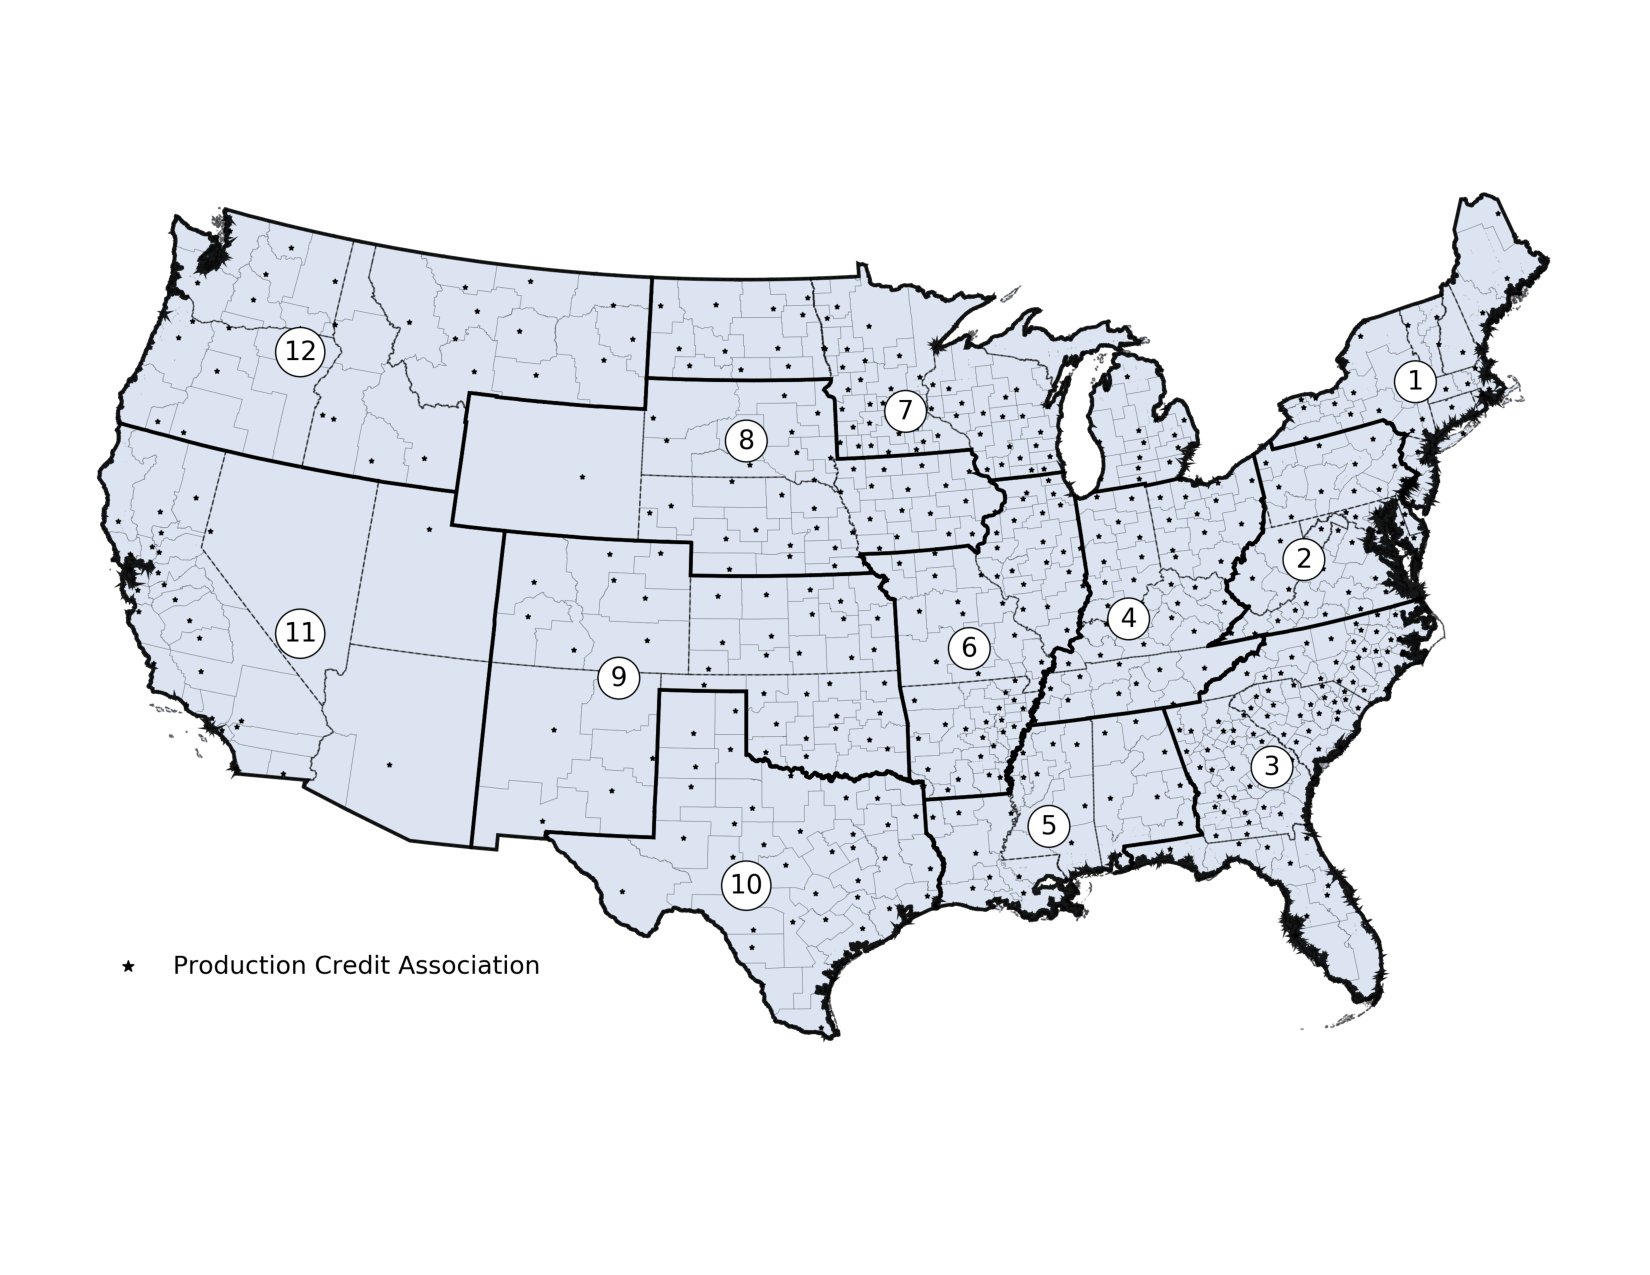
\includegraphics[width=1\textwidth]{PCA_districts}
\label{coverage_area}
Source: \citet{pca_location}

\footnotesize Note: darker lines are district boundaries, lighter lines are coverage area boundaries, stars are PCAs.
\end{figure}


By 1934, more than 500 associations across the country had together lent about 130,000 loans totaling around 107 million dollars, meaning on average loans were less than one hundred dollars. 
As late as 1946, only seven percent of the six million farmers belonged to PCAs and PCA lending was only 14\% of loan volume by commercial banks \citep{Arnold1958}. 
While their initial reach was modest, they were an important source of credit in many areas.
PCAs provided 20\% of production loans among Florida citrus growers in 1940, and 44\% of short-term lending in North Carolina in 1940 \citep{Reitz1942,Lange1944}. 
Notably, studies showed that merchant credit use in South Carolina and Arkansas fell 20 to 30 percentage points from 1926 to 1938 \citep{Sparlin1940,Moore1929,Ferrier1940,wickens_agricultural_1931}.
According to one South Carolina merchant, the decrease in their business was directly attributable to the actions of PCAs:

\begin{quote}
He stated that he couldn't conduct a credit business as he once did, that people have changed, that farmers are able to get money more readily from other sources than formerly and are preferring to pay cash, and that the user will borrow from a bank or production credit association to pay the store bill rather than make an annual fall settlement. \citep[pg. 35]{Ferrier1940}
\end{quote}

Even if at the national level their reach was small, there is evidence that PCAs had a meaningful impact on some areas of the country.
Farmers owned the PCAs, which meant the PCAs likely had a natural advantage in monitoring and screening farmer lenders as is typical with cooperative enterprises \citep{hueth2015agents,smith_adverse_1990}. 
\citet{Arnold1958} mentions that the PCAs possessed this advantage in alleviating asymmetric information.
 Since the PCAs could serve customers commercial banks ``would not'' lend to, it is likely that the PCAs actually played a complementary role to commercial banks.
 This is consistent with what \citet{alston_why_1994} finds, that is that FCS banks were complementary to commercial banks by capturing borrowers viewed as too risky by commercial banks.

How meaningful were these institutions to the farmers following the agricultural crisis of the early 1920s and the bank failures of 1929?
Understanding the answer to this question helps us understand the unique contribution that the GSE model has made to agriculture and its importance as an institutional innovation in credit markets.
In the next section, I discuss the sorts of factors that would determine the effect of PCAs on agricultural outcomes in the years following the agricultural crisis.

\section*{Conceptual Framework}

What is the effect of credit rationing on economic outcomes?
In the \citet{Bencivenga1993} model, low risk borrowers are offered less credit by lenders to prevent attracting high risk borrowers. 
Since low-risk projects are rationed out of the market, credit rationing decreases both output and capital. 
In the case of agriculture, information issues cause rationing to small farmers or tenant farmers if their projects are viewed as riskier than those of large farms \citep{carter_equilibrium_1988,stiglitz_credit_1981}. 
Small farms must then rely on ``signaling'' by either owning capital or belonging to a producer association to get a loan \citep{hoff_introduction:_1990}.

One of the consequences of credit rationing in agriculture can be lower than optimal use of inputs into production and consequently lower yields \citep{carter_impact_1989,foltz_credit_2004}.
At this critical time in US agriculture, a lack of credit to small farms could have seriously inhibited farm growth by reducing the adoption of inputs such as fertilizer and machinery.
The introduction of PCAs would have lessened these constraints and led to increases in crop yield and input use through three mechanisms: increased input use, knowledge transfer, and pro-competitive effects on interest rates. 
Understanding the first mechanism is the main goal of the analysis. 
The last two are fruitful directions for research, but are beyond the scope of this paper.

Upon the introduction of PCAs, farmers likely used their production credit to increase input use.
PCAs specialized in production credit that was short-term and was typically used for operating expenses.
As the access to production credit could allow households to use more inputs, this would consequently affect crop yield through its effect on inputs.
In the empirical analysis, I analyze use of fertilizers and tractors as examples of inputs that may increase because of access to production credit.
Increased liquidity in the household via production credit can be used to both buy variable inputs and also free up funds for farmers to invest in capital like machinery.

PCAs may affect crop yield through two other mechanisms: social learning and interest rate competition. 
Extension agents and other FCS staff were reportedly involved with the operations of PCAs, so access to technical expertise was likely another benefit of borrowing from a PCA. 
Introducing a PCA could raise crop yields if their cooperative structure facilitated information sharing among farmers.
PCAs may have also impacted the financial markets by bringing down the interest rates of commercial bank loans \citep{murray_agricultural_1941}.
PCA interest rates were capped at seven percent which may have forced some banks and input merchants to lower their interest rates to compete with PCAs.
Discerning these mechanisms requires more data on the PCAs and the markets they entered into, both of which are beyond the scope of this current analysis.

\begin{figure}
    \centering
    \caption{Directed Acyclic Graph of Distance and Outcomes}
    \label{DAG}
    \quad \\
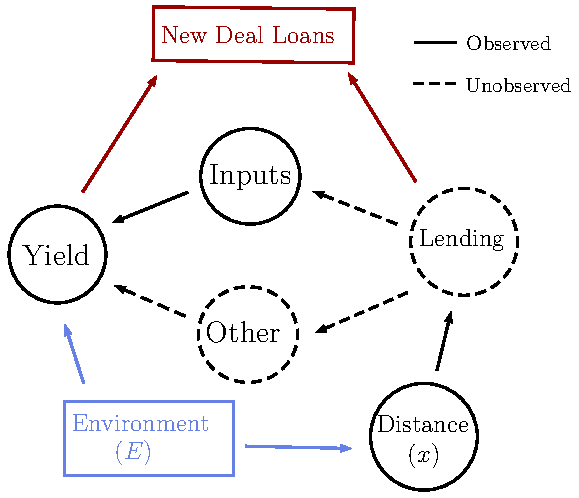
\includegraphics[width=.5\textwidth]{DAG.pdf}

\footnotesize
Note: Blue boxes represent examples of confounding variables, red boxes of bad controls.
\end{figure}

Figure \ref{DAG} shows a directed acyclic graph (DAG) representing the relationship between county distance to a PCA (``Distance'') and county input use (``Inputs'') and crop yield (``Yield'').
Since we only observe the location of the PCA and not its lending, distance is the only observable proxy for actual lending to farms.
Distance is inversely related to lending because banks tend to lend to the counties closest to them \citep{agarwal2010distance,degryse2005distance}.
This is especially true in the 1930s when poor rural infrastructure made traveling more costly than in today's context.
Lending is expected to then influence either inputs, which we observe, or ``Other,'' which are factors such as learning or effects on interests rates of other banks. 
Lending should be positively associated with yield through both of these channels.

Figure \ref{DAG} also shows two examples of confounding factors and bad controls.
The confounding factor example is pre-treatment environment, which could include soil characteristics, climate, or other factors that would influence yields and PCA placement.
Factors that suggest crop profitability (e.g. favorable soil) are likely correlated to both yield and PCA placement, making them confounding factors that should be used as controls.
By this same logic, we may also want to control for New Deal programs which may have targeted poorly performing areas and are also related to PCA placement.
However, certain New Deal loan programs are undesirable as controls because they are potentially influenced by the PCA placement.
Many of these programs start in 1933 and go throughout 1939, meaning decisions about funds happened after PCAs were already placed.
If a PCA is actively lending in an area, this likely would have influenced the need for New Deal loan programs in that same area.
Since these loan programs may have been targeted to low-yield areas, it is also reasonable to believe that yields would have influenced the programs.
Given these two directions of potential causality, variables like the New Deal loan programs are endogenous controls.

All three of these mechanisms suggest one direction for a relationship: the existence of a PCA should have increased crop yields and use of inputs.
Unlike other government loan programs, the PCAs are not as likely to attenuate productivity through encouraging the survival of low-productivity farms.
Alleviating credit rationing tends to lead to higher productivity since potentially profitable projects are now being offered credit \citep{Bencivenga1993}. 
Since PCAs would still consider their own credit risks when lending, there is no reason to necessarily believe that low-productivity farms would receive credit as they might in a less discriminating government loan program.

In the empirical model, I look at the effect of PCA distance on five outcomes: corn yield, wheat yield, crop value per acre, tractors per farm, and fertilizer per acre.
The first three examine the impact on yield directly while the last two examine the link to input use.
Examining inputs directly helps tease out the first mechanism, while examining crop yield directly helps us to understand the total effect. 
In the next section, I present the data and identification strategy for teasing out the relationships displayed in Figure \ref{DAG}.

\section*{Data}
To examine the impacts of PCAs on agricultural outcomes, I use county-level data from the US Agricultural Census, grid-level data on various environmental factors, and historical data on New Deal Spending, bank deposits, and PCA locations.
The primary dataset I use is the US Agricultural Census from 1920-1940 collected by \citet{haines_united_2016}. 
I chose this period to obtain two rounds of data before the establishment of the PCAs in 1933 while not including potentially confounding policy effects that happened after 1940 (including structural changes in the Farm Credit Administration and the beginning of World War II). 
The census contains county-level data on crops planted, crops harvested, total number of farms and other farm characteristics such as tractor and fertilizer use.

The environmental controls include measures of soil productivity, soil erosion, temperature, and precipitation.
For soil productivity, I use suitability measurements for rain-fed corn and wheat from the Global Agro-ecological Zones spatial dataset available at \citet{fao}.
The GAEZ suitability measures use data on terrain conditions, temperature, and other climate measures to estimate the potential production of different crops throughout the world.
I extract the average GAEZ suitability for rainfed corn and wheat across the whole county as a proxy measure for soil productivity.
Because the study period coincides with the Dust Bowl, a significant shock to the agricultural sector, I use erosion map data from \citet{hornbeck_enduring_2012} to control for areas that would have been disproportionately affected by dust storms in the late 1930s. 
Temperature and precipitation for each census year comes from \citet{prism} and is measured at the annual level (average for temperature, sum for rainfall).
Each county-level measurement is the average of the gridded cells within that county using the 1920 county boundaries \citet{nhgis}.

To address both the widespread bank failures as well as New Deal programs, I draw on two sources of historical data.
First, I use New Deal spending data available from \citet{fishback_can_2003} to measure spending programs that may have impacted agricultural output and input use and were targeted to similar counties as the PCAs (e.g. the agricultural adjustment act (AAA) payments). 
This data is only available as a sum total of the years 1933-1939, and so in this analysis is a time-invariant variable.
Second, I use a dataset of bank deposits and suspensions during the years 1920-1937 from the FDIC to control for differential access to credit across the US \citep{fdic_1992}.
Since many PCAs were formed to directly address lack of access to credit, it is important to take into account which counties lost the most deposits in the 1929 crisis as a potential confounding variable.
I extract the percentage of bank deposits suspended between 1929 and 1933 for each county as a measure of pre-treatment exposure to bank failure.

\subsection*{\textit{PCA Locations}}
PCA locations in the period 1935-1940 and their coverage areas are available from a map of their locations in 1937 obtained from the US National Archives and Records Administration (see Figure \ref{coverage_area}).\footnote{Because only about three percent of banks closed between 1935 and 1940, their location in 1937 largely reflects where they were in 1935 and 1940, though admittedly with some error.} 
Similar to \citet{kantor_research_2019} and \citet{altonji2005evaluation}, I use the distance from each county centroid to the city where its ``serving PCA'' was located to proxy for access to PCA credit. 
Since PCAs were not allowed to lend outside their coverage areas, this is the most relevant distance for examining impact. 
Distance to a bank has been shown to negatively impact credit access \citep{agarwal2010distance,degryse2005distance}, and would have inhibited access even more in the 1930s.
In the first decade of PCA operation, counties further away from their ``coverage area'' were typically not served:

\begin{quote}
Checks on the location of borrowers after 2 or 3 years of operation almost invariably showed that most of the business was within the home county or at least relatively near the association headquarters. 
Service in the more distant areas was not satisfactory and a large percentage of the farmers living there had no knowledge about the associations. \citep[pg. 50.]{Arnold1958}
\end{quote}

Over time, this became less and less the case as the PCAs established ``field offices'' to reach farmers that were more distant from the main office. 
In the first five or ten years of operation, the probability of getting a loan from a PCA was strongly affected by whether a farm was in a county close to the PCA office or not.
This is further motivation to not extend the analysis past 1940, since distance to the main office is unlikely to be the main determinant of credit access after field offices were established.
When exploring the effect of distance over discrete levels, I bin distance into rough quintiles of 30 kilometers, 45 kilometers, 60 kilometers, and 100 kilometers.\footnote{While not strictly quintiles of the distribution, the bins were chosen to be more economically meaningful. For example, given that a typical car in the 1930's could go roughly 60 kilometers per hour on a highway, these bins represent half hour, forty five minutes, and hour traveling times.}

\begin{figure}
    \centering
    \caption{PCA Bin Distances by County}
    \label{country_dist}
    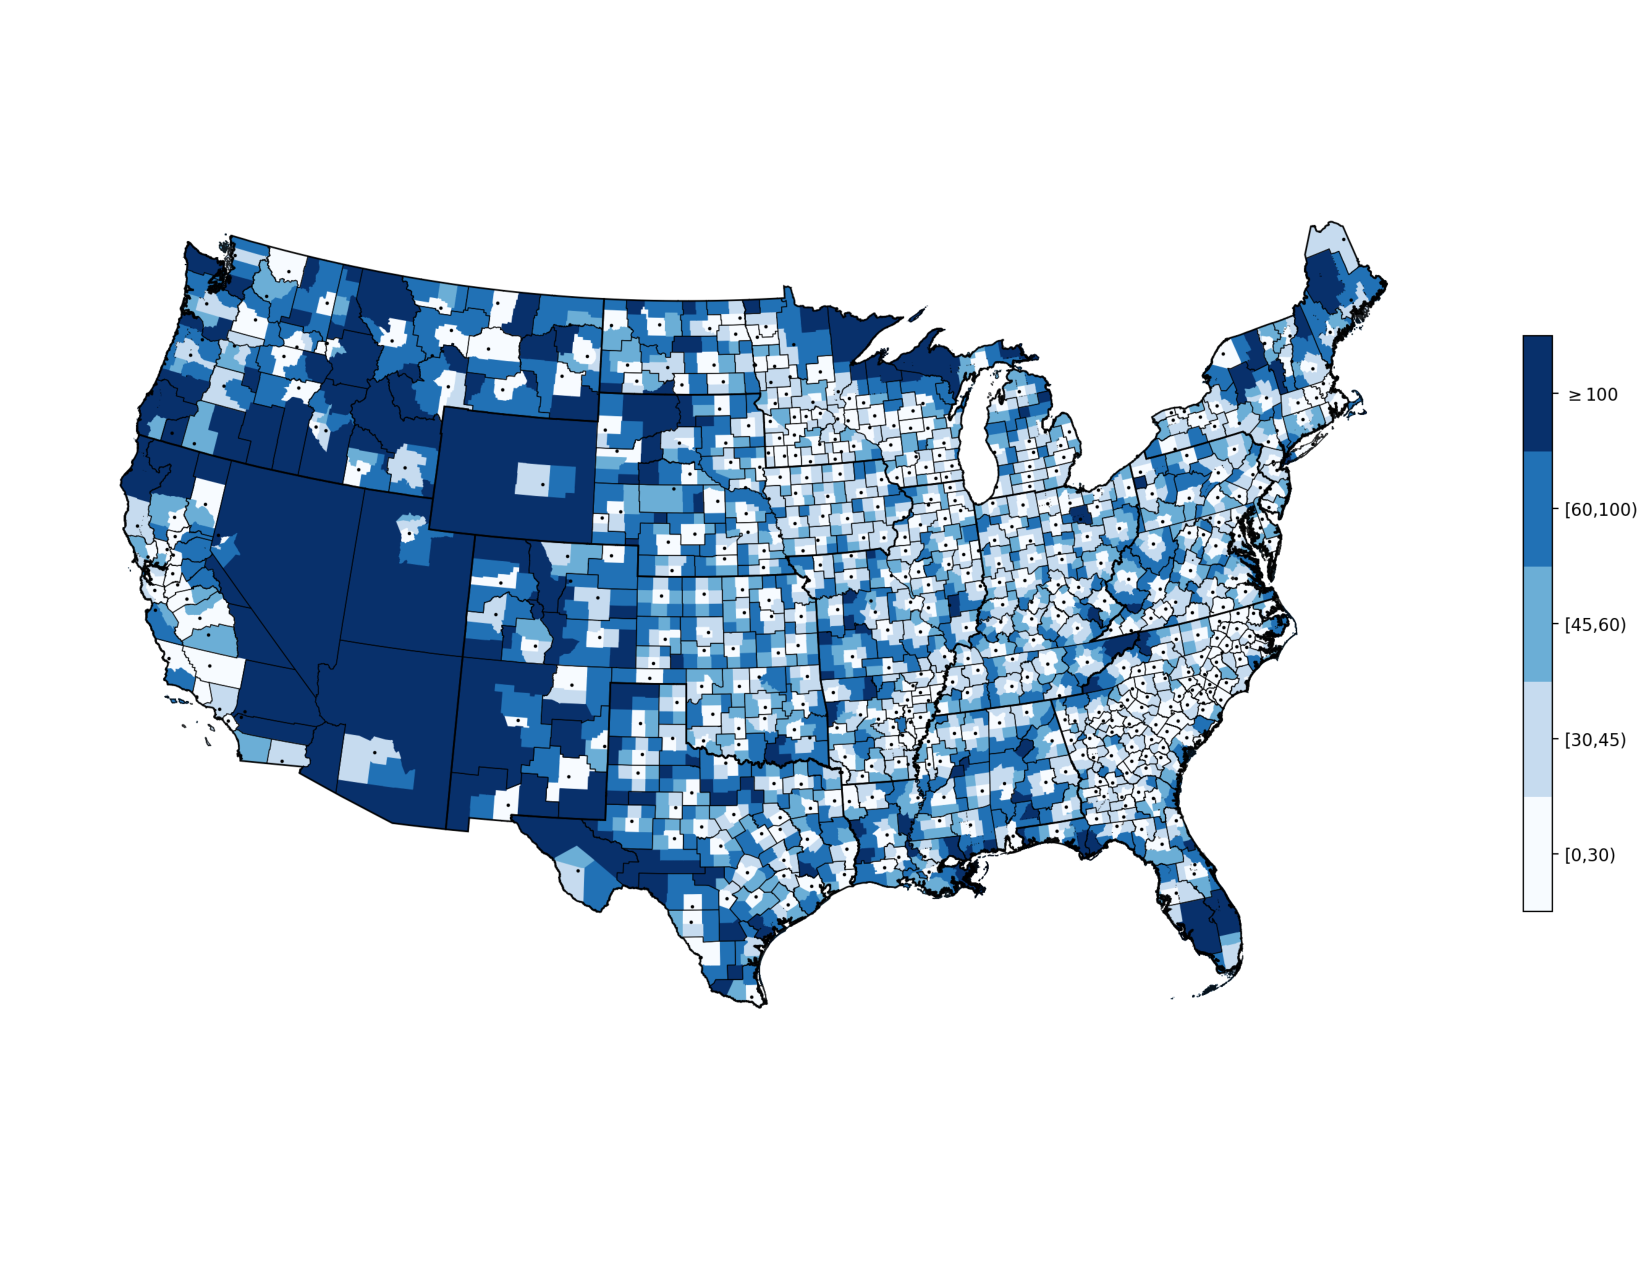
\includegraphics[width=1\textwidth]{Counties_Distance_from_PCA}\\
    Sources: \citet{pca_location}, own calculations.

    \footnotesize Note: darker lines are PCA coverage areas, dots are PCAs. \\
    Distances from county centroids to serving PCAs are measured in kilometers.
\end{figure}


Figure \ref{country_dist} shows the distance of each county from its serving PCA using the bins.
Note that the largest distances are in the western part of the country, where four states -- Arizona, Wyoming, Nevada, and Utah -- had only one PCA for the entire state.\footnote{These counties are later dropped as a robustness check. These results can be found in Figure \ref{sample_map} and Table \ref{crop_val_sample}.}
In the rest of the country, long distances are mostly driven by PCA coverage areas being drawn in such a way that some counties are far from their serving PCA, despite being close to other population centers (e.g. across the PCA coverage area border).
These counties serve as the main point of comparison for counties that either received a PCA or were drawn into a coverage area such that they were close to their serving PCA.

The PCA placement reflects both the need to increase credit access by having distances be short and the need to generate sufficient business by making the coverage areas large enough:

\begin{quote}
It had been determined that the area to be included in each association's territory should be \emph{as small as possible} for convenient service and, at the same time, of \emph{sufficient} size so that the fees and interest spread on the future volume of loans would pay expenses and provide some reserves for losses. \citep[pg. 29, emphasis added.]{Arnold1958}  
\end{quote}
These two conflicting goals would suggest that bank placement could introduce two sources of bias.
To garner enough business to stay solvent, PCAs may have been located in areas with a high amount of agricultural activity.
In estimation, this may make PCAs appear more effective than they actually are if these areas were already going to do well.
Conversely, it may also be that PCAs were placed in under-served areas that had lower amounts of agricultural activity.
This may make the PCAs appear to be less effective than they actually are.



\subsection*{County Agricultural Data}
How similar are counties far from PCAs compared to those close to PCAs?
To assess potential bias, I first examine trends in outcomes across different distance categories.
In addition to the five studied outcomes, I examine area in farms, number of farms, and average farm size across PCA distances in order to spot any trend differences between counties.
For corn and wheat yield, data is available for all five census years (1920, 1925, 1930, 1935, and 1940).
However, for crop value and fertilizer spending no information is available in 1935, and tractors were not measured in 1920 or 1935.
All yield measurements are divided by the amount of planted acres in the county, fertilizer is divided by the number of farm acres in the county, and tractors are divided by the number of farms.\footnote{Dividing number of tractors by farm area would indicate intensity of use, but here I focus instead on whether more farms owned tractors. For the latter, tractors by farm number is a more relevant measure}

I graph the averages of relevant variables across years and bins of distance in Figure \ref{trend_vars} and Figure \ref{trend_pacr}.
The variation across space is represented with multiple lines which represent the discrete distance bins from Figure \ref{country_dist}, with darker lines representing greater distance from the PCA.
In general, three events are important to remember when looking at these trends.
First, farm prices crashed in the early 1920s (evidenced by the dip in most graphs at this time).
Second, the PCAs were established in 1933 (indicated by a dashed vertical line).
Third, the Great Plains were hit by dust storms between 1934 and 1936 (evidenced by another dip in yields in 1935).
The Dust Bowl impacted wheat yields the most, since wheat was widely grown in the Great Plains region.
The last year in this sample is 1940, which is before changes brought on by World War II starting in late 1941.
In this time period, the PCAs could potentially have been a part of mitigating both the financial turmoil of the early 1930s and the environmental turmoil in the late 1930s.

Figure \ref{trend_vars} shows that counties close to PCAs had a different expansion path than counties far from PCAs.
Counties more than 100 km away have the lowest crop revenue but also show a trend of gradually increasing farm size.
Many of the counties farthest from PCAs were in the West, which was likely expanding in this period.
These further areas likely have more cattle operations that practice extensive grazing, which is supported by the fact that these areas also had the lowest total crop value.
For areas closer to PCAs, the trends in farm area and average farm size look very similar.
For example, the average farm size experienced almost no change between 1925 and 1930, and even tractor adoption appears to follow very similar rates of increase from 1925 to 1930 for these areas.

At all distances, there is a noticeable increase in the number of farms in 1935 and a decrease in an average farm size.
Part of this may be due to the increase in government payments which increased farm income by 50\% in 1935 compared to 1932 \citep{rasmussen1976short}.
After 1935, the number of farms goes back down, likely following the trend of consolidation that characterized farming after 1940. 
This 1935 shock is a reminder that any PCA effects measured in 1935 are the most likely to be confounded with government programs.

Figure \ref{trend_pacr} shows the trends in the studied outcomes, which are all adjusted for acreage and farm number.
Evidence of the Dust Bowl is clearest in the trends in wheat yields, which follow a decline in both 1935 and 1940.
For many of these outcomes, all the expansion paths across PCA distance look similar with the exception of the furthest counties.
The counties more than 100 km away from their serving PCA look fundamentally different in terms of their expansion paths.
These counties experienced large increases in fertilizer and crop value per acre relative to areas closest to PCAs from 1925 to 1930.
While counties close to PCAs had higher levels relative to farther areas, their prior trends are usually declining or increasing by less than other areas.
This may be a result of placing PCAs in places of high agricultural activity that were recovering the slowest.

These trends, however, are not conditioned on any of the confounding variables that might be correlated with PCA placement.
Also, it is not clear from these figures whether the PCAs had any measurable impact on these outcomes.
In the next section, I detail my empirical strategy for uncovering the impacts of PCAs on crop yield and input use.

\begin{figure}
    \centering
    \caption{Trends in Levels For Major Variables}
    \label{trend_vars}
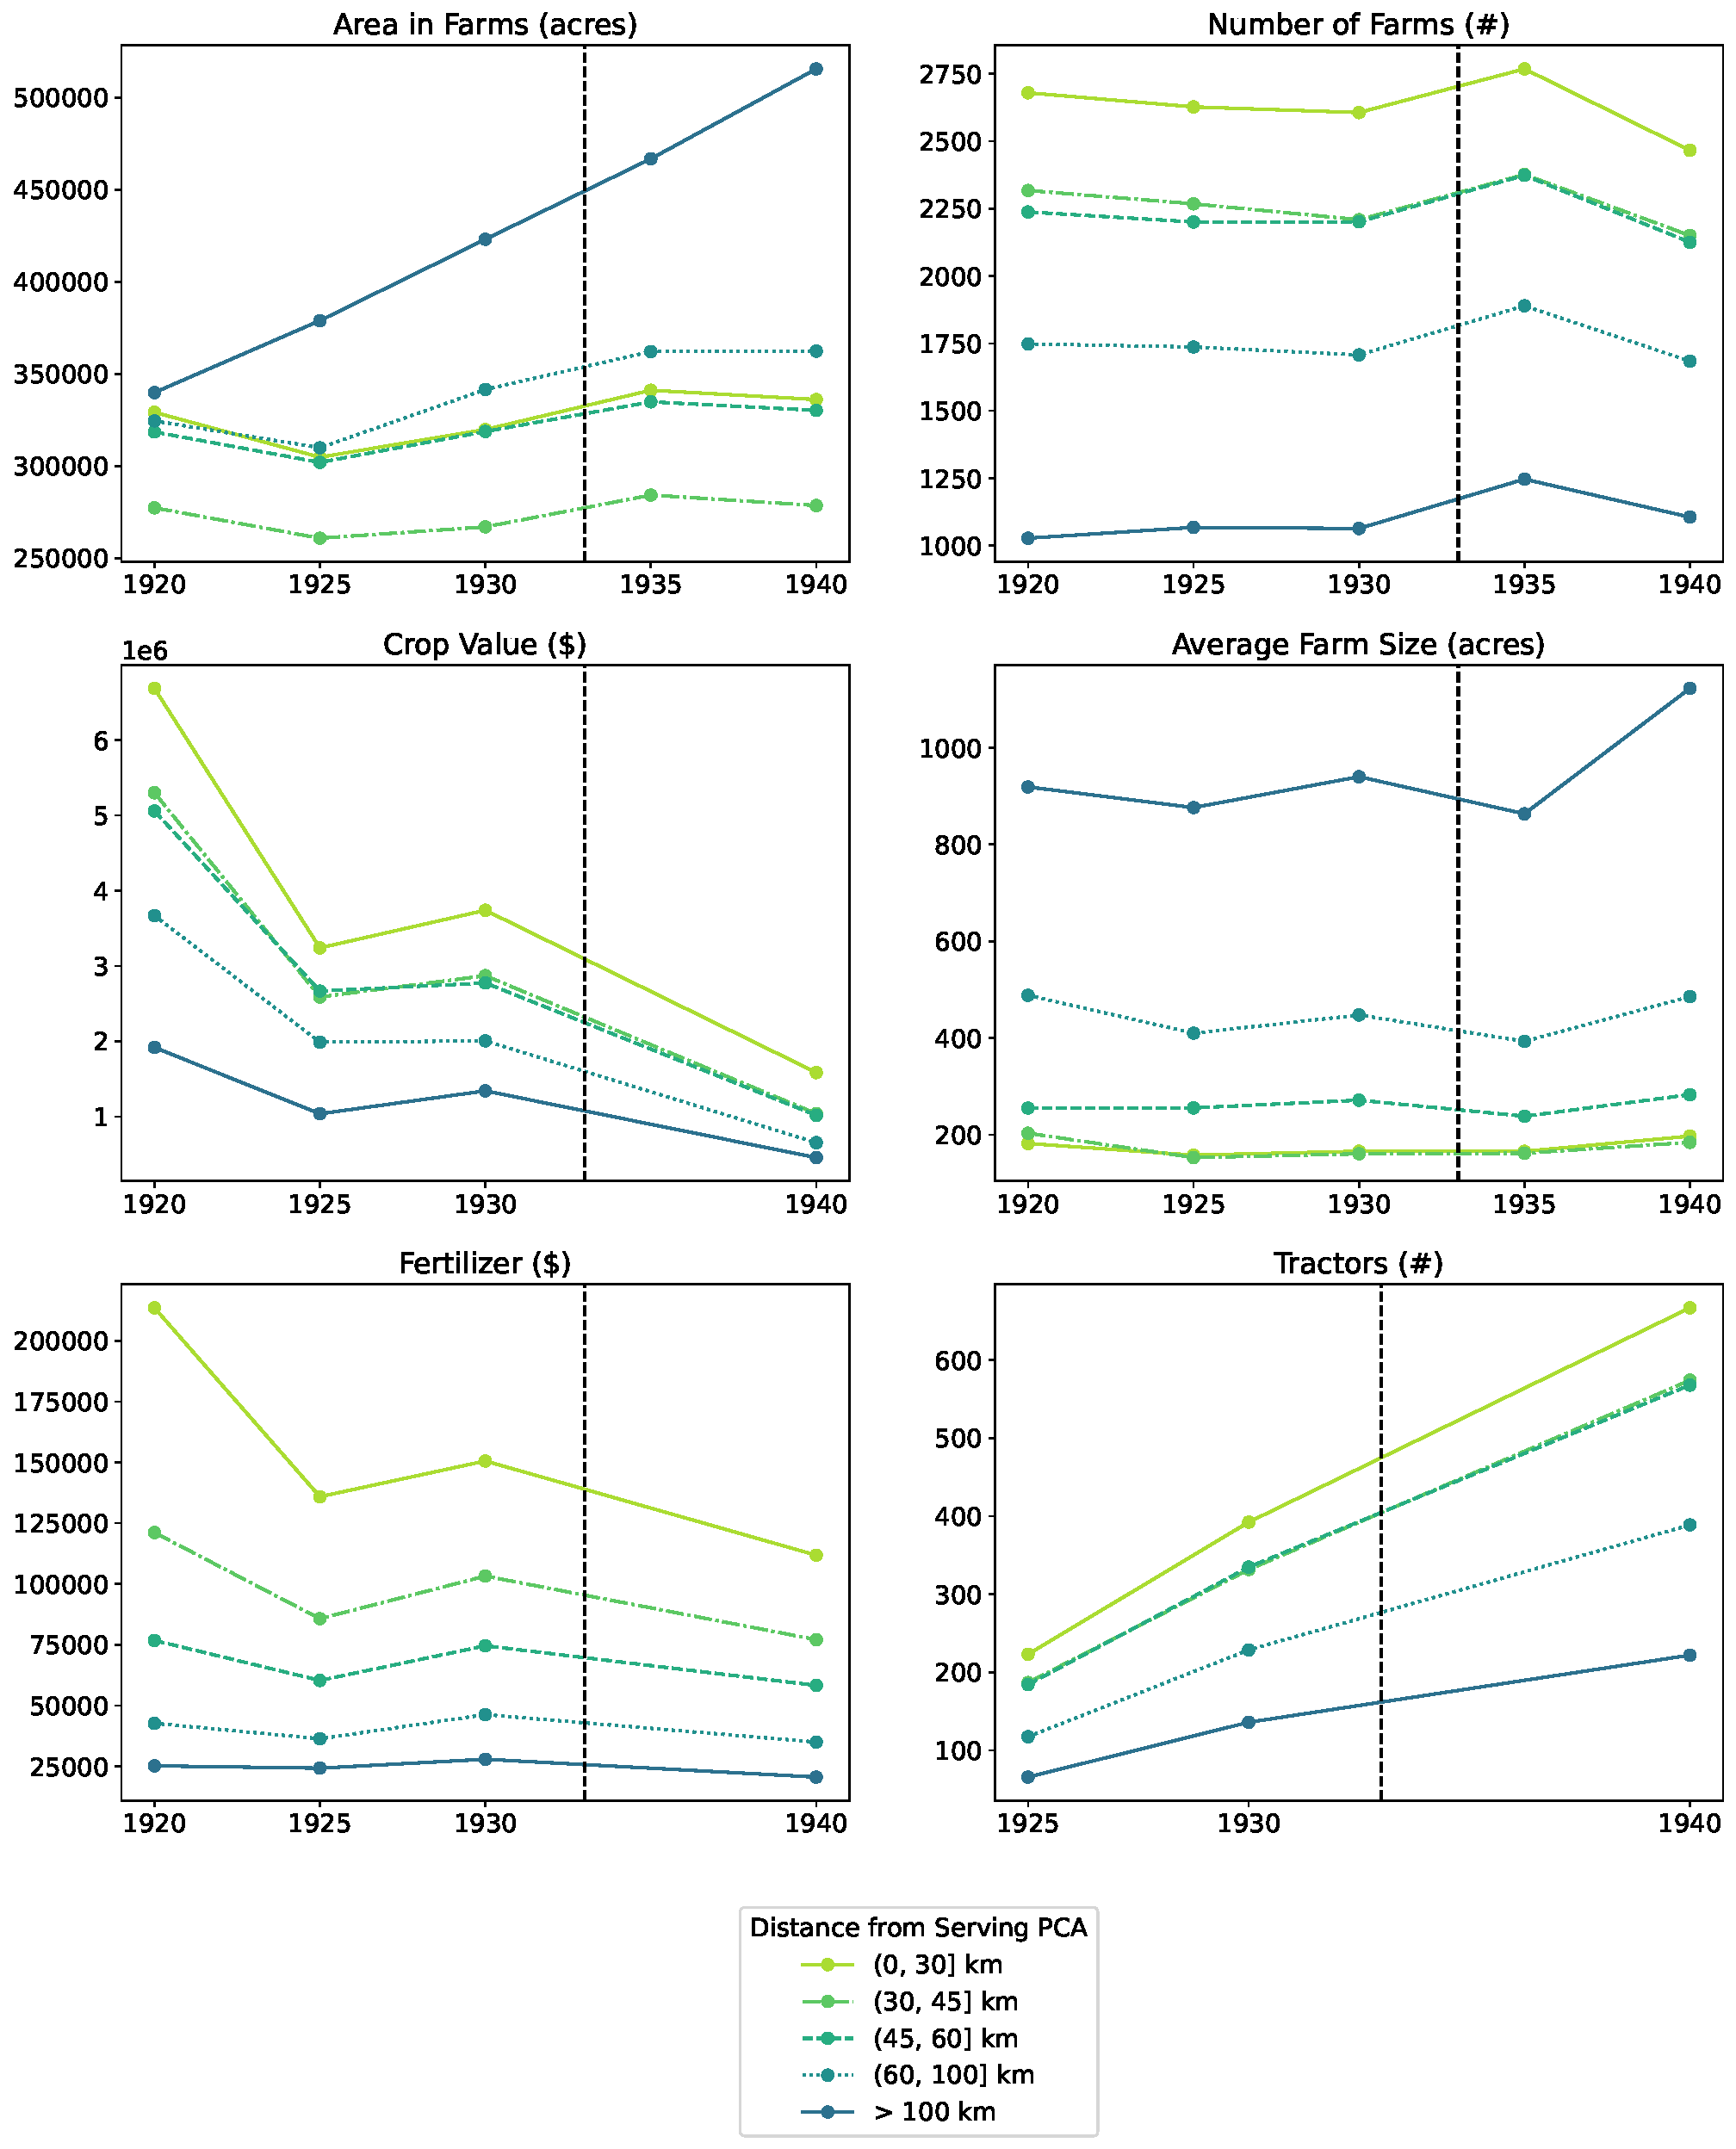
\includegraphics[width=1\textwidth]{trends_levels.pdf} \\
\footnotesize Note: each point estimate is the mean across counties in that distance category for that year.
\end{figure}

\begin{figure}
    \centering
    \caption{Trends in Outcomes}
    \label{trend_pacr}
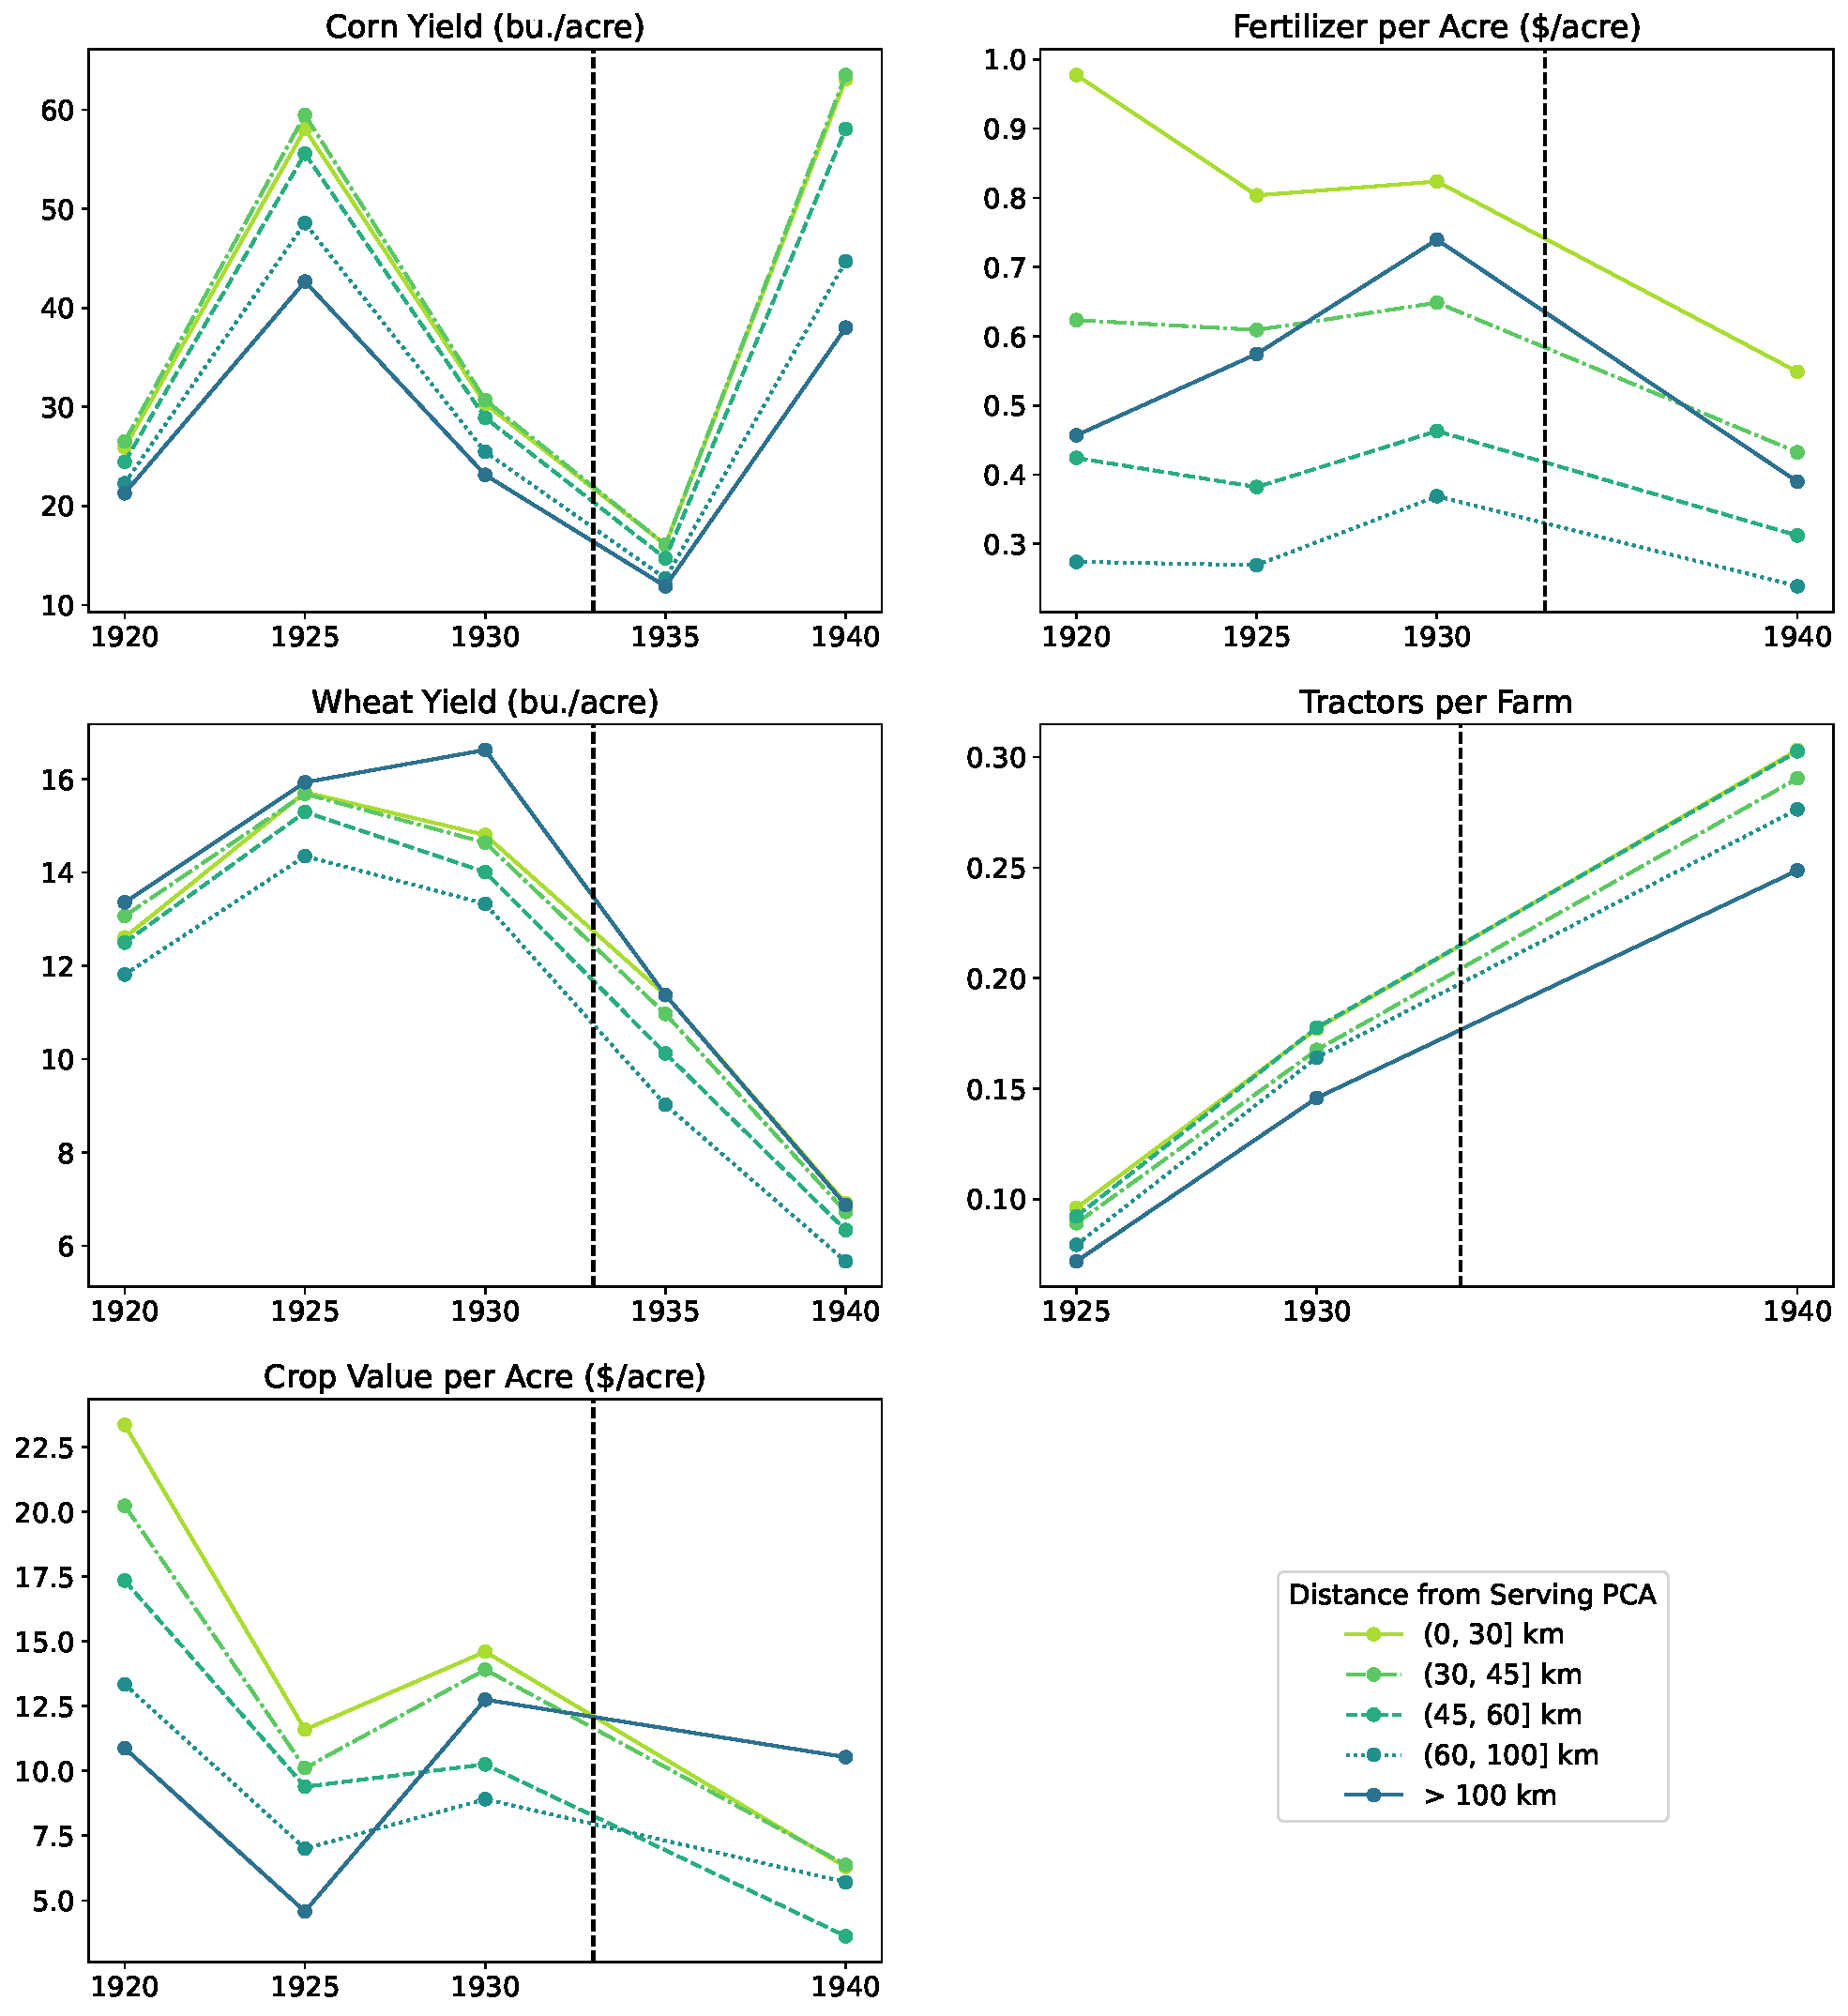
\includegraphics[width=1\textwidth]{trends_pacr.pdf} \\
\footnotesize Note: each point estimate is the mean across counties in that distance category for that year.

\end{figure}

\section*{Methodology}
To examine the short-run impact of the PCAs, I use the following specification:
\begin{align}
\label{equation:main}
IHS(Y_{it}) = \mu_i + \tau_t \gamma \mathbf{Z_{it}} + \sum^{1940}_{j=1920} \beta_j x_i \times \mathbbm{1}\{t=j\} + \delta_j \mathbf{E_i} \times \mathbbm{1}\{t=j\} + \epsilon_{it},
\end{align}
where:
\begin{itemize}
\item \textit{$Y_{it}$} is the outcome for county $i$ in period $t$,
\item \textit{$x_{i}$} is some function of distance to the serving PCA (either IHS transformed or binned),
\item \textit{$\mathbf{Z_{it}}$} is a vector time-varying control variables (temperature and rainfall),
\item \textit{$\mathbf{E_i}$} is a vector of time-invariant control variables (soil quality, New Deal Spending, erosion levels, lost deposits in 1929, etc.),
\item \textit{$\tau_t$} and \textit{$\mu_i$} are time and county fixed effects.\footnote{A full list of the covariates is found at the bottom of Table \ref{tab:full_sample}.}
\end{itemize}

 To account for occasional zero values of \textit{$Y_{it}$}, I use the inverse hyperbolic sine (IHS) transformation which can account for zeros but retain the interpretation of a log-transformed variable \citep{bellemare_elasticities_2020}. 
 Time-invariant variables \textbf{$\mathbf{E_i}$} are interacted with time fixed effects to allow different levels of these variables to have different time trends.
 The summation term $\sum^{1940}_{j=1920}$ indicates that there is an interaction between \textbf{$\mathbf{E_i}$} and year fixed effects for every sample year except the base period.
 This allows counties with different levels of pre-treatment characteristics to still have different time trend impacts.
 For example, counties with different levels of erosion may experience year effects differently due to environmental shocks which damaged only counties with high erosion.
Time-varying controls are limited to weather effects to avoid including endogenous controls.
Another set of included controls are state-by-year interaction to control for unobserved state policies during this time.
The standard errors for the model are clustered at the county level.

The estimates of interest are $\beta_{1935}$ and $\beta_{1940}$, which is the relationship of distance to PCA location with $Y$ after the PCAs were placed in 1933.
Since there were no PCAs in these locations in the years 1930, 1925 and 1920, it is expected that $\beta_{1925} = \beta_{1920} = 0$, meaning there is no statistically significant relationship between county outcomes and these locations otherwise.
The specification is an example of the two-way fixed effects (TWFE) estimator with multiple periods. 
Depending on whether $x_{i}$ is discrete or continuous, different assumptions need to hold for $\beta$ to be a reliable estimate of the average treatment effect on the treated (ATT), meaning the causal impact of the PCA placement on the areas that received PCAs.
Suppose that $x_i$ is a binary variable which equals 1 if the county is near a PCA:
\begin{align}
ATT = E(Y_{it}(1) - Y_{it}(0)|x_i=1)
\end{align}
where $Y_{it}(1)$ is the outcome of the group that received a PCA in 1933 and $Y_{it}(0)$ is the outcome of those that did not.
The important assumption that must hold for the TWFE estimate to be equivalent to the ATT is ``parallel trends'': that the changes in $Y$ in counties with and without PCAs would have been the same in the absence of PCA placement.
In other words, had the FCS not organized PCAs then those candidate counties would have had a parallel rate of growth to the counties who were not close to the PCA.
A number of time-invariant, pre-treatment characteristics may lead to a violation of parallel trends, which motivates the inclusion of covariates \textbf{$\mathbf{E_i}$} and \textbf{$\mathbf{Z_{it}}$} in the equation so that parallel trends need only hold conditional on these covariates.
The inclusion of covariates also necessitates a stronger assumption of the effects of covariates on $Y$, namely that the covariates also exhibit a type of parallel trends \citep{santanna_doubly_2020}.
This necessitates being judicious with how many covariates are included in the regression equation.\footnote{More specifically, \citet{santanna_doubly_2020} points out that two other things must hold in order to identify the ATT with covariates. 
It must be the case that i) treatment effects are homogenous in the covariates and ii) the effect of the covariates on $Y$ also exhibit a form of parallel trends whereby $E(Y_{it}(1) - Y_{it}(0)|x_i=1,\mathbf{Z_{it}}) = E(Y_{it}(1) - Y_{it}(0)|x_i=1)$ (in other words, no ``covariate-specific'' trends).}
Since using covariates makes it necessary to impose more assumptions to identify the ATT, I compare models with and without covariates in the Results section.

In what follows, treatment is defined as distance from the county centroid to the serving PCA and therefore either i) a continuous variable or ii) a sequence of binary variables representing the bins of distance.
Using a continuous treatment in a TWFE model is an approach found in similar analyses such as \citet{nunn_potatos_2011}, \citet{qian_missing_2008}, and most relevantly \citet{kantor_research_2019}.
\citet{kantor_research_2019} examines the effect of the placement of State Agricultural Experiment Stations on county-level crop yield and estimates the relationship between distance to the experiment station both before and after the stations were placed.
With multiple periods, this design results in a $\beta$ estimate for each year.
This significance of the ``pre-treatment period,'' in this case meaning 1925 and 1920, is often used as heuristic to provide evidence of parallel trends holding or being violated.
If distance has no effect before the PCAs are placed (1920 and 1925), then this is often considered evidence that parallel trends holds\footnote{Note that the significance of prior periods only tells us about parallel trends in a very specific case. It only informs us about parallel trends in the special case that the trend in a year like 1925 is assumed to be parallel in subsequent years (1930 and onward in this case). See pgs. 425-6 of \citet{cunningham_causal_2021} for an examination of this assumption.}

Unfortunately, using continuous distance presents its own issues.
If $x_i$ is a continuous variable, the coefficient $\beta$ represents the marginal effect \textit{at all levels of distance}.
For example, estimating an elasticity for all levels of distance must assume that the effect of traveling one kilometer 10 kilometers away from a PCA is equivalent to traveling one kilometer 100 kilometers away.
To allow for non-linear effects, the main specification uses binned distance using the cut-offs found in Figures \ref{trend_vars} and \ref{trend_pacr}.
This definition of treatment allows for treatment effects to be different at different levels of distance instead of assuming the effect of distance must be the same at every level of distance.
For example, we might expect that counties within 60 kilometers of a PCA experience similar levels of treatment, whereas counties farther than 60 kilometers could be past the distance threshold were service is possible.
The binned distance specification allows us to examine these kinds of non-linear effects, though I retain the more traditional approach using the continuous variable in order to ease comparison to other studies such as \citet{kantor_research_2019}.\footnote{One disadvantage of using a continuous treatment is that the TWFE estimator may not deliver the ATT the researcher desires, but may instead estimate a weighted average of ATTs across levels of the treatment. A recent working paper, \citet{callaway_difference--differences_2021}, examines the case in which a continuous variable is used as treatment in a difference-in-difference model. They find that the TWFE effect is a weighted average of ATTs when the treatment response is different at different levels of treatment. The bin estimator estimates these treatment responses in essence with several binary variables which have a more straightforward interpretation, but it is not clear how precisely this strategy related to \citet{callaway_difference--differences_2021}. In a later section, I compare the results of these strategies with a simple binary approach in order to have a baseline with more familiar assumptions.} 

Since the treatment is distance from the PCA, I expect that \textit{$\beta_{1935}$} and \textit{$\beta_{1940}$} will both be less than zero.
This would indicate that counties \textit{closer} to PCAs had \textit{higher outcomes} when compared to further counties in 1935 and 1940.
If access to credit through PCAs had a positive impact on any of these outcomes, the counties furthest from PCAs will have relatively \textit{lower} outcomes compared to those closest to PCAs.
Since we observe two census periods prior to placement, I can also test whether $\beta_{1920} = \beta_{1925} = 0$, an outcome consistent with parallel trends if the differences in 1925 would have persisted without PCAs.
The significance of these years also sheds light on the selection process of the PCAs and whether they targeted relatively well off or relatively worse off counties. 
For example, if $\beta_{1925}>0$, then areas \textit{far} from PCAs were \textit{better off} in these outcomes and areas \textit{close} to PCAs were relatively \textit{worse off}.
This suggests that PCAs were placed in areas that needed assistance as opposed to areas that were already well off.
If the prior years are assumed to be indicative of the trends the counties \textit{would have experienced}, then their significance also indicates the sign of the bias for TWFE from non-parallel trends.
If $\beta_{1925}<0$, this method would overestimate the impact of PCAs, whereas if $\beta_{1925}>0$ then this method would underestimate it.\footnote{\citet{cunningham_causal_2021} shows that a TWFE estimate in the two period case with two treatments can be decomposed as the ATT plus a ``non-parallel trends bias,'' which is the counterfactual trend of the treated group minus the counterfactual trend of the untreated group: $\hat{\beta} = ATT + [(E(Y_{T}(0)|Post) - E(Y_{T}(0)|Pre)) - (E(Y_{U}(0)|Post) - E(Y_{U}(0)|Pre))]$, where $T$ is treated and $U$ is untreated. If the prior period coefficients are assumed to be indicative of the counterfactual trend, then if the treated group has lower outcomes in the prior period relative to the untreated group this causes $\hat{\beta}$ to be lower than the actual ATT since $(E(Y_{T}(0)|Post) - E(Y_{T}(0)|Pre)) < (E(Y_{U}(0)|Post) - E(Y_{U}(0)|Pre)).$}
Intuitively, if distance has a negative effect \textit{before} PCAs were placed, then any negative effect found \textit{after} PCAs were placed is likely overstated.
A similar argument would follow if distance to PCA was positively related to these outcomes even before PCAs existed at those locations.


\section*{Results}
I estimate two versions of the empirical model: log-log and log-binned.
In the log-log model, both the outcome and the distance are IHS-transformed.
In the log-binned model, the outcome is IHS-transformed but the distance measure is represented as a series of bins where counties within 30 km of a PCA are the comparison group.
This last specification is used in all robustness checks, including those present in the Appendices.
For all specifications, the transformation explained in \citet{bellemare_elasticities_2020} is applied to allow the parameters to be interpreted as elasticities and percentage increases.\footnote{Specifically, the log-log coefficients are transformed such that the tables display the coefficient $\hat{\beta}$ multiplied by $\bar{x} (\sqrt{\bar{y}^2 +1})/(\bar{y} \sqrt{\bar{x}^2+1}))$, where $x$ is the distance measure and $y$ is the outcome. For the log-binned model, the coefficients are transformed using $exp(\beta) -1$, which is standard for the log-binary model.}
The base year is always 1930 and the base distance category is counties within 30 kilometers of their PCA.
The effects of the covariates are omitted from these tables, but an explanation of the covariates and their effects on the outcomes can be found in Appendix \ref{appendix:covars}.

\begin{table}\centering
    \caption{PCA Distance and Agricultural Activity}
    \label{log-log}
Log Distance Model

\footnotesize   
\vspace{.5cm} 
% Negative coefficients indicate a positive association \\
% between PCA proximity and agricultural outcomes.\\
Base category: Year $=$ 1930
\def\sym#1{\ifmmode^{#1}\else\(^{#1}\)\fi}

\begin{threeparttable}[t]
\begin{tabular}{l*{3}{c}}
    \hline\hline
 & \multicolumn{3}{c}{\textbf{Crop Yield}} \\

                    &\multicolumn{1}{c}{IHS(Corn Yield)}&\multicolumn{1}{c}{IHS(Wheat Yield)}&\multicolumn{1}{c}{IHS(Crop Value/Acre)} \\
\hline
1920 $\times$ IHS(PCA Distance)& 0.005          & 0.017$^{***}$& $-$0.005             \\
                               & (0.006)        & (0.006)      & (0.007)              \\
                               &                &              &                      \\
1925 $\times$ IHS(PCA Distance)& $-$0.005       & 0.014$^{**}$ & $-$0.012             \\
                               & (0.008)        & (0.006)      & (0.008)              \\
                               &                &              &                      \\
1935 $\times$ IHS(PCA Distance)& $-$0.021$^{**}$& $-$0.003     &                      \\
                               & (0.008)        & (0.010)      &                      \\
                               &                &              &                      \\
1940 $\times$ IHS(PCA Distance)& $-$0.024$^{**}$& 0.009        & $-$0.037$^{***}$     \\
                               & (0.009)        & (0.008)      & (0.010)              \\
                               &                &              &                      \\
\hline
Observations                           &     13,929 & 13,277 & 11,292                   \\
Number of Clusters &2,823 &2,823 &2,823 \\
Adjusted $R^{2}$                          & 0.786 & 0.765 & 0.881                   \\
% Pre-Trend F stat & 0.6 & 1.664 & 0.771  \\ 
% Pre-Trend p-value & 0.549 & 0.19 & 0.463 \\ 
\hline\hline
& \multicolumn{3}{c}{\textbf{Inputs}} \\
&\multicolumn{1}{c}{IHS(\# Tractors/Farm)} &           \multicolumn{1}{c}{IHS(\$ Fert/Acre)} & \\ \hline
1920 $\times$ IHS(PCA Distance)&                 & 0.004   & \\
                               &                 & (0.008) & \\
                               &                 &         & \\
1925 $\times$ IHS(PCA Distance)& 0.002           & 0.002   & \\
                               & (0.006)         & (0.006) & \\
                               &                 &         & \\
1940 $\times$ IHS(PCA Distance)& $-$0.040$^{***}$& $-$0.002& \\
                               & (0.008)         & (0.007) & \\
                               &                 &         & \\
                               \hline
Observations &  8,469 & 11,165 &  \\ 
Number of Clusters &2,823 &2,823 & \\
Adjusted R$^{2}$  & 0.926 & 0.963 & \\ 
% Pre-Trend F-test  & 0.084 & 0.124 & \\ 
% Pre-Trend P-Value & 0.772 & 0.883 & \\ 
\hline
\end{tabular}
    \begin{tablenotes}
        \item {\footnotesize * \(p<0.10\), ** \(p<0.05\), *** \(p<0.01\). Standard errors clustered at the county-level.}
        \item{\footnotesize \textbf{Time-varying controls:} average annual temperature (mean of cells within county), average annual temperature squared, annual total precipitation, annual total precipitation squared.}
        \item {\footnotesize \textbf{Time-invariant controls:} GAEZ corn and wheat soil potential (average of cell), suspended deposits in 1929, erosion levels, total relief spending, total public works spending, and total grants. Details on these New Deal spending variables can be found in \citet{fishback_can_2003}.}
        \item {\footnotesize All specifications include county, year, and state-by-year fixed effects.}
        \item {\footnotesize New Deal spending variables are the sum of the years 1933-1939 and suspended deposit data is from the period 1929-1933. }
    \end{tablenotes}
\end{threeparttable}
\label{tab:full_sample}
\end{table}



Table \ref{log-log} shows the elasticities calculated from the model where both the outcome and distance are IHS transformed.
The ``pre-treatment'' coefficients are the years 1920 and 1925 and the ``post-treatment'' coefficients are 1935 and 1940.
For every outcome except wheat yield, the distance is not statistically significant to the outcome prior to 1935.
For wheat, they are positive in the pre-treatment period, meaning PCAs were located farther from high wheat yielding areas.
In the post-treatment period, corn yield, crop value, and tractors have a negative and statistically significant relationship with distance to a PCA.
After 1930, areas closer to PCAs had higher corn yield (0.02 elasticity), higher crop value per acre (0.037 elasticity), and higher tractors per farm (0.04 elasticity).
While statistically different than zero, these elasticities are much smaller than for example the effects of experiment stations measured by \citet{kantor_research_2019} (about 0.2 elasticity).


\begin{table}
    \centering

    \caption{PCA Distance and Agricultural Activity}
Binned Distance Model

\footnotesize   
\vspace{.5cm} 
% Negative coefficients indicate a positive association \\
% between PCA proximity and agricultural outcomes.\\
Base category: Year $=$ 1930 and $<$ 30 km from a PCA
    \label{log-bin}
    \begin{threeparttable}[t]
    \footnotesize


\begin{tabular}{lcccccc}
\hline\hline
% & \multicolumn{6}{c}{} \\
& \multicolumn{6}{c}{\textbf{Crop Yield}} \\
[.5em]
&\multicolumn{3}{c}{IHS(Corn Yield)}&\multicolumn{3}{c}{IHS(Wheat Yield)}\\
[.5em]
\cline{2-7}
& & & & & & \\ 
& \multicolumn{1}{c}{} & \multicolumn{2}{c}{\textbf{Post-Treatment}} & \multicolumn{1}{c}{} & \multicolumn{2}{c}{\textbf{Post-Treatment}} \\
Distance from PCA     & 1925 & 1935 & 1940 & 1925 & 1935 & 1940 \\ \hline
$[30, 45)$ km & 0.006    & $-$0.054$^{**}$ & $-$0.031        & 0.025        & $-$0.044    &  $-$0.014    \\
              & (0.027)  & (0.025)         & (0.029)         & (0.020)      & (0.031)     &  (0.029)     \\
              &          &                 &                 &              &             &              \\
$[45, 60)$ km & 0.007    & $-$0.068$^{**}$ & $-$0.010        & 0.045$^{*}$  & $-$0.051    &  0.011       \\
              & (0.032)  & (0.030)         & (0.035)         & (0.025)      & (0.036)     &  (0.034)     \\
              &          &                 &                 &              &             &              \\
$[60, 100)$ km& 0.012    & $-$0.089$^{***}$& $-$0.089$^{**}$ & 0.069$^{***}$& $-$0.032    &  $-$0.007    \\
              & (0.032)  & (0.032)         & (0.035)         & (0.025)      & (0.036)     &  (0.032)     \\
              &          &                 &                 &              &             &              \\
$>$ 100 km    & $-$0.019 & $-$0.120$^{*}$  & $-$0.137$^{**}$ & 0.026        & $-$0.008    &  0.063       \\
              & (0.067)  & (0.062)         & (0.062)         & (0.041)      & (0.054)     &  (0.055)     \\
         [1em]
         \hline
         Obs      &   \multicolumn{3}{c}{13,929}  &   \multicolumn{3}{c}{13,277} \\
         Adj. $R^2$ &  \multicolumn{3}{c}{0.786} &\multicolumn{3}{c}{0.765}  \\

\hline\hline
% & \multicolumn{6}{c}{} \\
 &\multicolumn{2}{c}{\textbf{Crop Yield}} & \multicolumn{4}{c}{\textbf{Inputs}} \\
[.5em]

&\multicolumn{2}{c}{IHS(Crop Value per Acre)} &\multicolumn{2}{c}{IHS(\# Tractors/Farm)} &   \multicolumn{2}{c}{IHS(\$ Fert/Acre)} \\
[.5em]
\cline{2-7} 
& & & & & & \\
& \multicolumn{1}{c}{} & \multicolumn{1}{c}{\textbf{Post-Treatment}} & \multicolumn{1}{c}{} & \multicolumn{1}{c}{\textbf{Post-Treatment}} & \multicolumn{1}{c}{} & \multicolumn{1}{c}{\textbf{Post-Treatment}}  \\
Distance from PCA & 1925 & 1940 & 1925 & 1940 & 1925 & 1940                                                \\
\hline
$[30, 45)$ km & $-$0.026   &$-$0.024        & $-$0.026   & $-$0.009$^{**}$  & $-$0.005    & $-$0.002   \\
              & (0.026)    &(0.028)         & (0.026)    & (0.004)          & (0.012)     & (0.014)    \\
              &            &                &            &                  &             &            \\
$[45, 60)$ km & $-$0.003   &$-$0.072$^{**}$ & $-$0.003   & $-$0.010$^{**}$  & $-$0.005    & $-$0.014   \\
              & (0.024)    &(0.032)         & (0.024)    & (0.004)          & (0.014)     & (0.017)    \\
              &            &                &            &                  &             &            \\
$[60, 100)$ km& $-$0.043   &$-$0.146$^{***}$& $-$0.043   & $-$0.020$^{***}$ & $-$0.005    & $-$0.005   \\
              & (0.026)    &(0.030)         & (0.026)    & (0.004)          & (0.014)     & (0.016)     \\
              &            &                &            &                  &             &            \\
$>$ 100 km    & 0.017      &$-$0.181$^{***}$& 0.017      & $-$0.039$^{***}$ & 0.039$^{*}$ & $-$0.0002  \\
              & (0.049)    &(0.044)         & (0.049)    & (0.007)          & (0.020)     & (0.031)    \\
      [1em] \hline 
      Obs      &     \multicolumn{2}{c}{11,292} & \multicolumn{2}{c}{8,469} & \multicolumn{2}{c}{11,165} \\
      Adj. $R^2$ &  \multicolumn{2}{c}{0.882} & \multicolumn{2}{c}{0.926} & \multicolumn{2}{c}{0.963}\\
\end{tabular}
\begin{tablenotes}
    \item {\footnotesize * \(p<0.10\), ** \(p<0.05\), *** \(p<0.01\). Standard errors clustered at the county-level.}
    \item{\footnotesize \textbf{Time-varying controls:} average annual temperature (mean of cells within county), average annual temperature squared, annual total precipitation, annual total precipitation squared.}
    \item {\footnotesize \textbf{Time-invariant controls:} GAEZ corn and wheat soil potential (average of cell), suspended deposits in 1929, erosion levels, total relief spending, total public works spending, total grants, and total loans. Details on these New Deal spending variables can be found in \citet{fishback_can_2003}.}
    \item {\footnotesize All specifications include county, year, and state-by-year fixed effects.}
    \item {\footnotesize New Deal spending variables are the sum of the years 1933-1939 and suspended deposit data is from the period 1929-1933. }
    \end{tablenotes}
\end{threeparttable}
\end{table}

Table \ref{log-bin} explores non-linear impacts of distance by examining the bins of distance.
For each specification, the prior period 1925 is shown plus 1935 and 1940.\footnote{Distance in the year 1920 held no predictive power in these models and so is omitted for space reasons. In subsequent tables, I include an F-test of the hypothesis that the 1925 and 1920 coefficients are all zero.}
Just as in Table \ref{log-log}, wheat yield is the only outcome that bears a relationship to distance prior to 1935.
The coefficients are positive, confirming the areas further from PCAs prior to PCA placement had higher yields.
In the post-treatment period, wheat yields are not impacted by the presence of a PCA.
In contrast, county corn yields are lower in areas further from PCAs in 1935 and 1940.
Compared to counties within 30 km of a PCA, yields were between five to twelve percent lower in 1935.
In 1940, the differences between the base category and closer counties gradually disappears but persists for counties more than 60 km away from their PCA.
Crop value per acre is between seven and 18 percent lower compared to counties close to their PCA, with the largest effects being at the greatest distance.
Tractors exhibit the same pattern but with smaller effects: between a one and a four percent difference in tractor use per farm.
In all specifications, increased distances have a larger magnitude of impact, which is consistent with proximity to the PCA location being associated with higher outcomes.

\begin{table}
    \centering

    \caption{Binned Distance Model, Crop Value and Controls}
\label{crop_val_controls}

\footnotesize   
\vspace{.5cm} 
% Negative coefficients indicate a positive association \\
% between PCA proximity and agricultural outcomes.\\
Base category: Year $=$ 1930 and $<$ 30 km from a PCA

1940 Coefficients Only

\begin{threeparttable}[t]
\begin{tabular}{@{\extracolsep{5pt}}lccccc} 
    \\[-1.8ex]\hline 
    \hline \\[-1.8ex]
    \\[-1.8ex] & \multicolumn{5}{c}{Crop Value per Acre} \\ [.5em]
    \cline{2-6} 
    \\[-1.8ex] Distance from PCA & (1) & (2) & (3) & (4) & (5)\\ 
    \hline \\[-1.8ex] 
    $(30, 45]$ km & $-$0.093$^{***}$ & $-$0.079$^{***}$ & $-$0.072$^{***}$ & $-$0.071$^{***}$ & $-$0.024 \\ 
    & (0.030) & (0.026) & (0.026) & (0.026) & (0.028) \\ 
    & & & & & \\ 
    $(45, 60]$ km & $-$0.156$^{***}$ & $-$0.115$^{***}$ & $-$0.116$^{***}$ & $-$0.115$^{***}$ & $-$0.072$^{**}$ \\ 
    & (0.035) & (0.031) & (0.030) & (0.030) & (0.032) \\ 
    & & & & & \\ 
   $(60, 100]$ km & $-$0.284$^{***}$ & $-$0.201$^{***}$ & $-$0.200$^{***}$ & $-$0.198$^{***}$ & $-$0.146$^{***}$ \\ 
    & (0.027) & (0.027) & (0.027) & (0.027) & (0.030) \\ 
    & & & & & \\ 
   $>$ 100 km & $-$0.276$^{***}$ & $-$0.265$^{***}$ & $-$0.242$^{***}$ & $-$0.237$^{***}$ & $-$0.181$^{***}$ \\ 
    & (0.037) & (0.040) & (0.041) & (0.041) & (0.044) \\ 
    & & & & & \\ 
    Year by State FE &  & X & X & X & X \\ 
    Time-Invariant Controls &  &  & X & X & X \\ 
    Time-Variant Controls &  &  &  & X & X \\ 
    New Deal Spending &  &  &  &  & X \\ 
    \hline \\[-1.8ex] 
    Observations & 11,292 & 11,292 & 11,292 & 11,292 & 11,292 \\ 
    Adjusted R$^{2}$ & 0.814 & 0.869 & 0.871 & 0.871 & 0.882 \\ 
    Pre-Trend F-Statistic & 1.256 & 0.476 & 0.628 & 0.702 & 0.589 \\ 
    Pre-Trend p-value & 0.262 & 0.874 & 0.755 & 0.69 & 0.788 \\ 
    \hline 
    \hline \\[-1.8ex] 

\end{tabular}
\begin{tablenotes}
    \item {\footnotesize * \(p<0.10\), ** \(p<0.05\), *** \(p<0.01\).}
    \item {\footnotesize Standard errors clustered at the county-level.}
    % \item{\footnotesize \textbf{Time-varying controls:} average annual temperature (mean of cells within county), average annual temperature squared, annual average precipitation, annual average precipitation squared.}
    % \item {\footnotesize \textbf{Time-invariant controls:} GAEZ corn and wheat soil potential (average of cell), suspended deposits in 1929, erosion levels, AAA payments, FCA payments. Details on the New Deal spending variables can be found in \citet{fishback_can_2003}.}
    \item {\footnotesize All specifications include county, year, and state-by-year fixed effects.}
    \item {\footnotesize Pre-Trend F-test hypothesis is that $\beta_{1920} = \beta_{1925}=0$.}

    % \item {\footnotesize New Deal spending variables are the sum of the years 1933-1939 and suspended deposit data is from the period 1929-1933. }
    \end{tablenotes}
\end{threeparttable} 
\end{table}




\begin{table}
\centering

\caption{Binned Distance Model, Tractors and Controls}
\label{tractor_controls}

\footnotesize   
\vspace{.5cm} 

Base category: Year $=$ 1930 and $<$ 30 km from a PCA

1940 Coefficients Only

\begin{threeparttable}[t]
\begin{tabular}{@{\extracolsep{5pt}}lccccc} 
\\[-1.8ex]\hline 
\hline \\[-1.8ex]
\\[-1.8ex] & \multicolumn{5}{c}{Tractors/Farm} \\ [.5em]
\cline{2-6} 
\\[-1.8ex] Distance from PCA & (1) & (2) & (3) & (4) & (5)\\ 
\hline \\[-1.8ex] 
$(30, 45]$ km & $-$0.003        & $-$0.012$^{***}$& $-$0.012$^{***}$& $-$0.011$^{***}$& $-$0.009$^{**}$ \\
              & (0.006)         & (0.004)         & (0.004)         & (0.004)         & (0.004) \\
              &                 &                 &                 &                 & \\
$(45, 60]$ km & $-$0.002        & $-$0.014$^{***}$& $-$0.014$^{***}$& $-$0.013$^{***}$& $-$0.010$^{**}$ \\
              & (0.007)         & (0.005)         & (0.005)         & (0.004)         & (0.004) \\
              &                 &                 &                 &                 & \\
$(60, 100]$ km& $-$0.014$^{**}$ & $-$0.023$^{***}$& $-$0.024$^{***}$& $-$0.025$^{***}$& $-$0.020$^{***}$ \\
              & (0.006)         & (0.004)         & (0.004)         & (0.004)         & (0.004) \\
              &                 &                 &                 &                 & \\
$>$ 100 km    & $-$0.027$^{***}$& $-$0.041$^{***}$& $-$0.047$^{***}$& $-$0.047$^{***}$& $-$0.039$^{***}$ \\
              & (0.008)         & (0.007)         & (0.007)         & (0.007)         & (0.007) \\
              &                 &                 &                 &                 & \\
Year by State FE &  & X & X & X & X \\ 
Time-Invariant Controls &  &  & X & X & X \\ 
Time-Variant Controls &  &  &  & X & X \\ 
New Deal Spending &  &  &  &  & X \\ 
\hline \\[-1.8ex] 
Observations          & 8,469 & 8,469 & 8,469 & 8,469 & 8,469 \\ 
Adjusted R$^{2}$      & 0.786 & 0.901 & 0.903 & 0.911 & 0.926 \\ 
Pre-Trend F-Statistic & 0.97 & 1.131 & 1.07 & 1.626 & 0.244 \\ 
Pre-Trend p-value     & 0.423 & 0.34 & 0.37 & 0.165 & 0.913 \\ 
\hline 
\hline \\[-1.8ex] 

\end{tabular}
\begin{tablenotes}
\item {\footnotesize * \(p<0.10\), ** \(p<0.05\), *** \(p<0.01\).}
\item {\footnotesize Standard errors clustered at the county-level.}
% \item{\footnotesize \textbf{Time-varying controls:} average annual temperature (mean of cells within county), average annual temperature squared, annual average precipitation, annual average precipitation squared.}
% \item {\footnotesize \textbf{Time-invariant controls:} GAEZ corn and wheat soil potential (average of cell), suspended deposits in 1929, erosion levels, AAA payments, FCA payments. Details on the New Deal spending variables can be found in \citet{fishback_can_2003}.}
\item {\footnotesize All specifications include county, year, and state-by-year fixed effects.}
\item {\footnotesize Pre-Trend F-test hypothesis is that $\beta_{1920} = \beta_{1925}=0$.}

% \item {\footnotesize New Deal spending variables are the sum of the years 1933-1939 and suspended deposit data is from the period 1929-1933. }
\end{tablenotes}
\end{threeparttable} 
\end{table}


Tables \ref{crop_val_controls} and \ref{tractor_controls} examine the impact of different levels of controls on crop value per acre and tractor use.
In lieu of displaying pre-trends, each table includes an F-test testing the hypothesis that $\beta_{1920}=\beta_{1925}=0$ for all distance categories.
For all of these specifications, the hypothesis could not be rejected.
Using only the TWFE approach with no covariates, the estimates range from nine percent for counties 30-45 km away to 27\% for counties more than 100 km away.
The inclusion of controls reduces the magnitude of the change for all distance categories, leaving the most conservative estimate to be about 7-18\% change depending on proximity.
Including New Deal spending has one of the largest impacts on the coefficients.
After including spending, counties within 30-45 km away from a PCA are not statistically different to counties within 30 km.
Nevertheless, the differences persist for counties more than 45 km away.
The tractor outcome is much less influenced by including New Deal Spending and only slightly reduced in magnitude.

A large portion of counties farther than 100 km from their PCA are located in the West where farms are fundamentally different (see Figure \ref{country_dist}).
It is possible that these counties are driving the significance of the farthest distance category in predicting outcomes.
It is also possible that the results are being driven by counties hit by the dust storms in 1935, and so the results do not generalize to the rest of the country.
To examine the influence of these counties, I estimate the impact of distance on crop value per acre across different samples.
The counties in each sample are shown in Figure \ref{sample_map}.




\begin{figure}[ht]
    \caption{Robustness Check Samples}
    \label{sample_map}
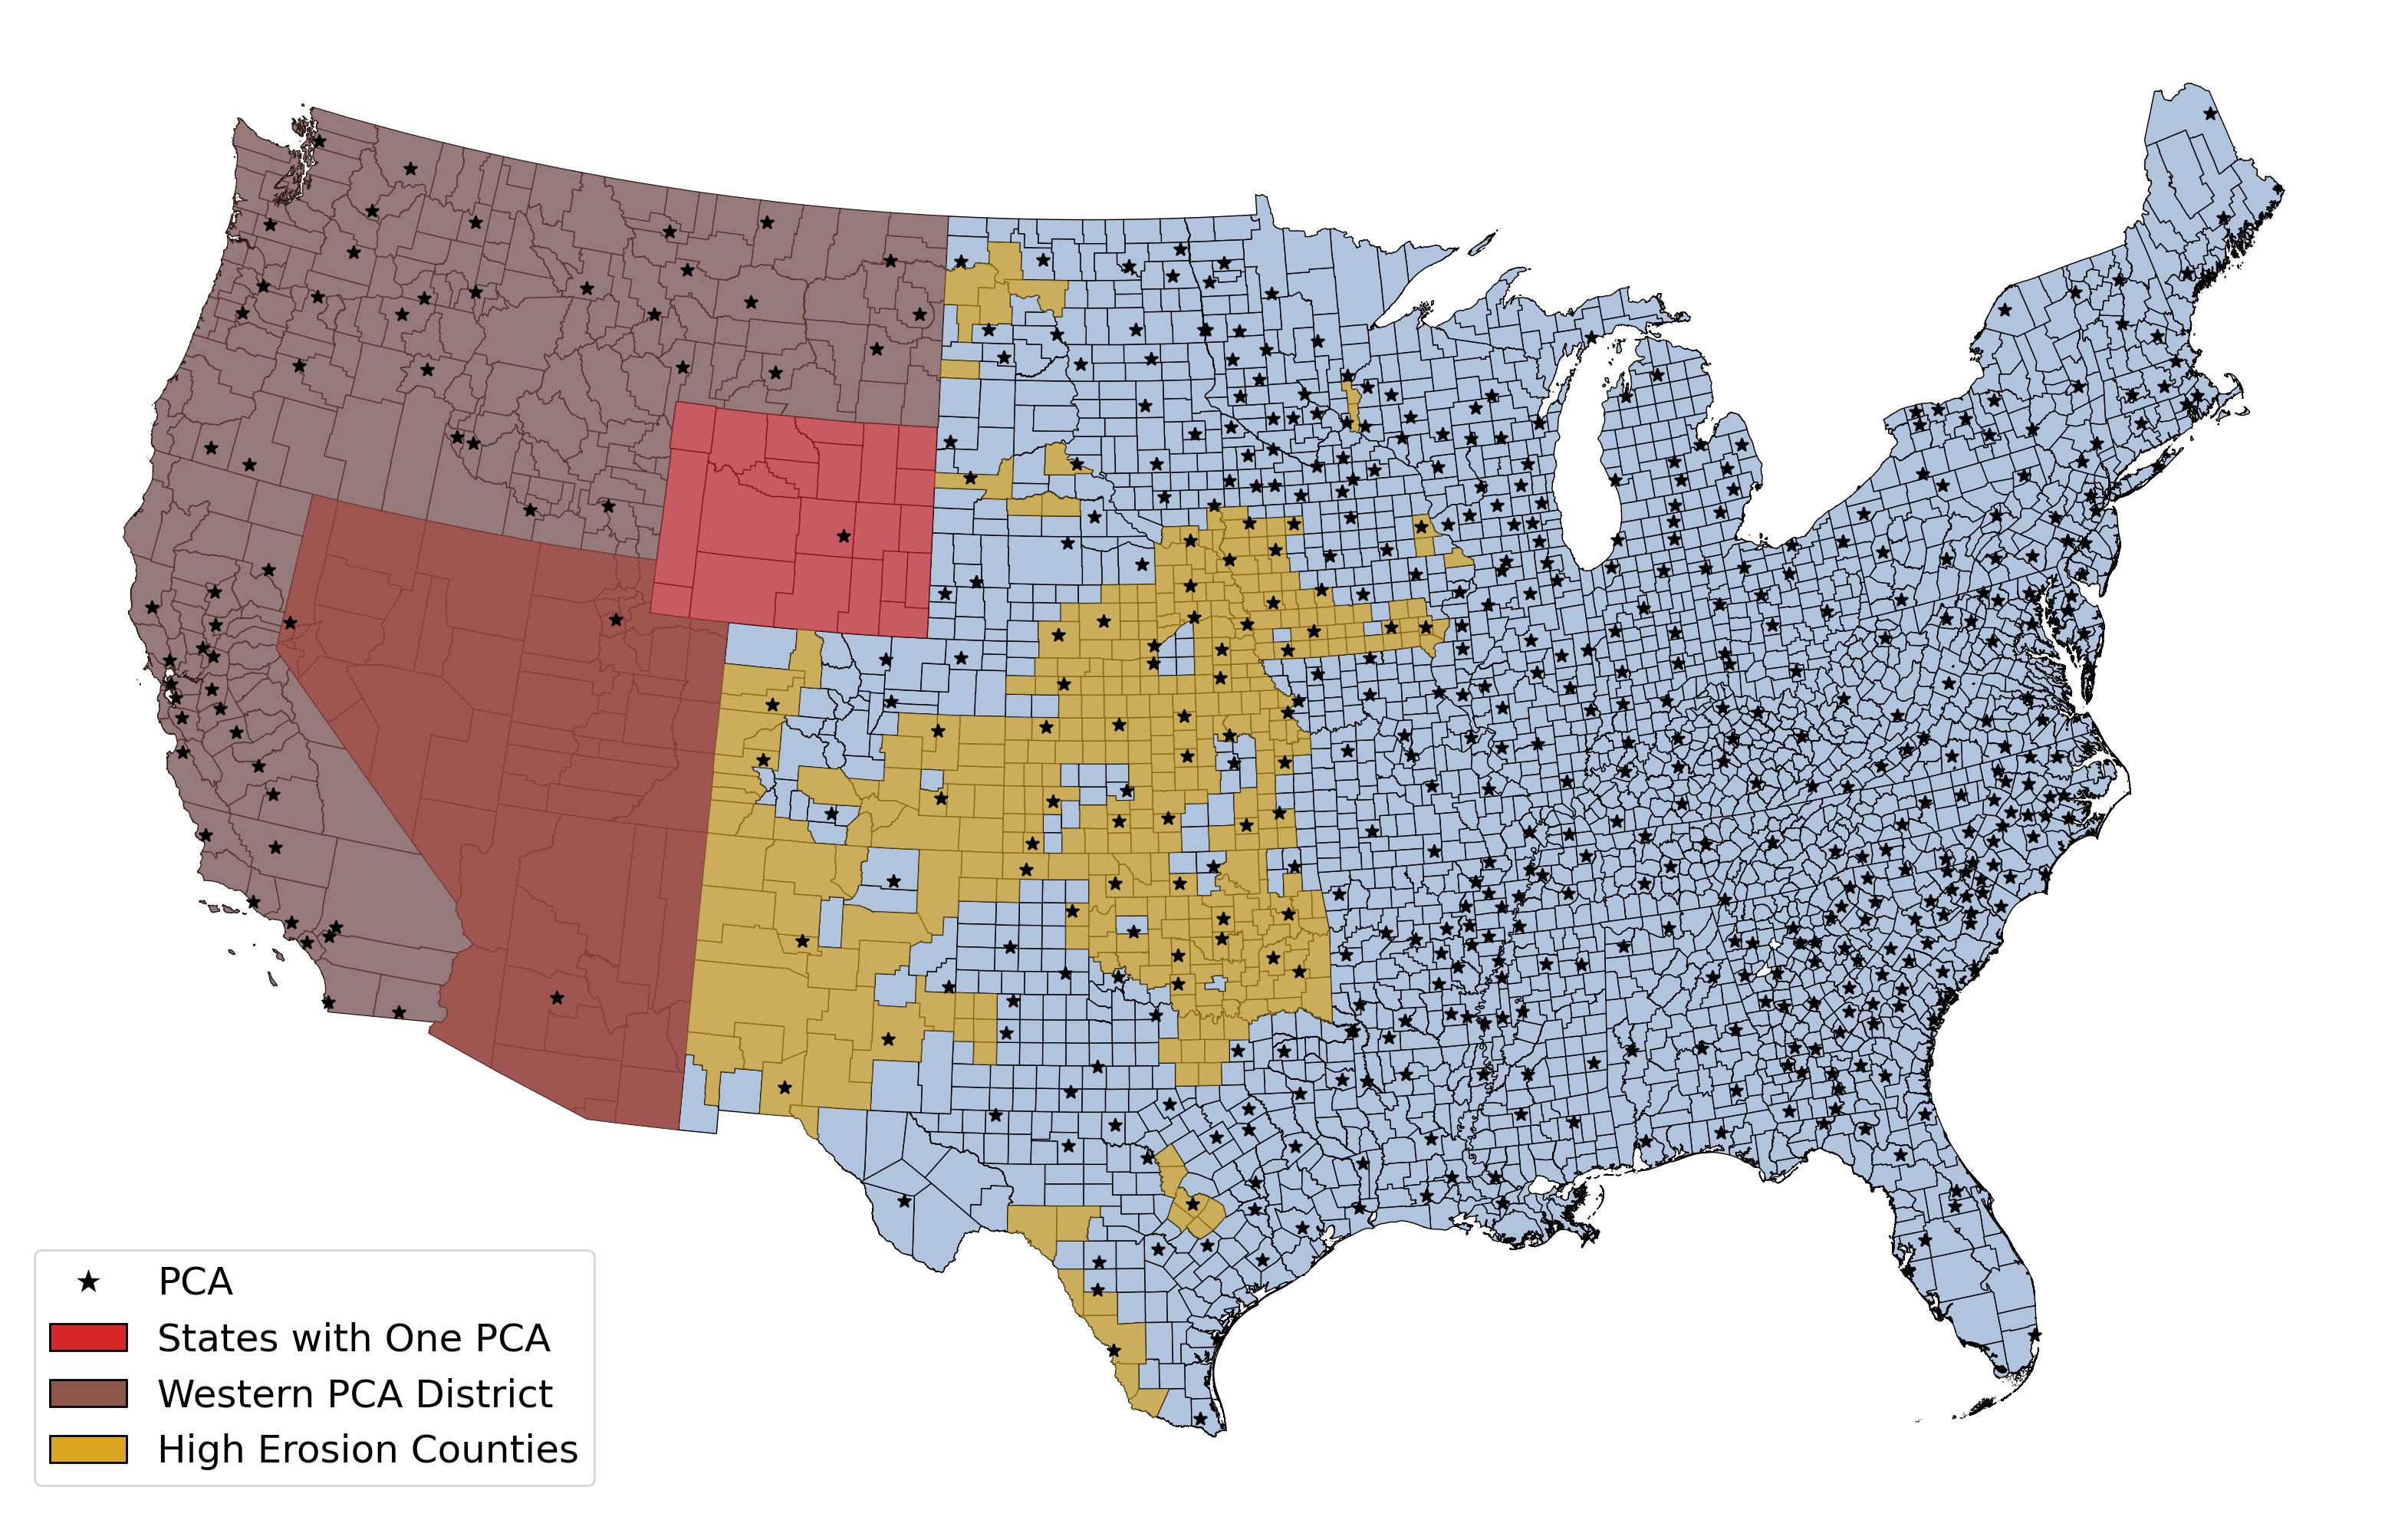
\includegraphics[width=\textwidth]{sample_map.png}
\end{figure}

\begin{table}
    \centering

    \caption{Binned Distance Model, Robustness Check Samples}
\footnotesize   
\vspace{.5cm} 
% Negative coefficients indicate a positive association \\
% between PCA proximity and agricultural outcomes.\\
Base category: Year $=$ 1930 and $<$ 30 km from a PCA

1940 Coefficients
\label{crop_val_sample}
\begin{threeparttable}[t]

\begin{tabular}{@{\extracolsep{5pt}}lccccc} 
    \\[-1.8ex]\hline 
    \hline \\[-1.8ex] 
    & \multicolumn{5}{c}{Crop Value per Acre} \\ 
    \cline{2-5} 
    \\[-1.8ex] & \multicolumn{5}{c}{} \\ 
    Distance from PCA & All Data & No States & No West & No Dust Bowl & Only Dust Bowl \\
             &           & With One PCA & & & \\ 
    \hline \\[-1.8ex] 
    $(30, 45]$ km & $-$0.022 & $-$0.030 & $-$0.036 & $-$0.009 & $-$0.094 \\ 
    & (0.028) & (0.027) & (0.027) & (0.029) & (0.095) \\ 
    & & & & & \\ 
    $(45, 60]$ km & $-$0.074$^{**}$ & $-$0.080$^{***}$ & $-$0.089$^{***}$ & $-$0.081$^{**}$ & $-$0.018 \\ 
    & (0.031) & (0.031) & (0.031) & (0.035) & (0.111) \\ 
    & & & & & \\ 
    $(60, 100]$ km & $-$0.145$^{***}$ & $-$0.151$^{***}$ & $-$0.164$^{***}$ & $-$0.147$^{***}$ & $-$0.138 \\ 
    & (0.030) & (0.029) & (0.030) & (0.036) & (0.101) \\ 
    & & & & & \\ 
    $> 100$ km & $-$0.179$^{***}$ & $-$0.200$^{***}$ & $-$0.157$^{***}$ & $-$0.227$^{***}$ & 0.021 \\ 
    & (0.044) & (0.042) & (0.049) & (0.058) & (0.146) \\ 
    & & & & & \\ 
    \hline \\[-1.8ex] 
    Observations & 11,292 & 11,088 & 10,400 & 9,924 & 1,368 \\ 
    Adjusted R$^{2}$ & 0.881 & 0.879 & 0.878 & 0.882 & 0.888 \\
    Pre-Trend F Stat & 0.644 & 0.558 & 0.624 & 0.872 & 0.601 \\ 
    Pre-Trend P-Value & 0.741 & 0.813 & 0.758 & 0.539 & 0.777 \\ 

    \hline 
    \hline \\[-1.8ex]
\end{tabular} 
 
    \begin{tablenotes}
        \item {\footnotesize * \(p<0.10\), ** \(p<0.05\), *** \(p<0.01\).}
        \item {\footnotesize Standard errors clustered at the county-level.}
        % \item{\footnotesize \textbf{Time-varying controls:} average annual temperature (mean of cells within county), average annual temperature squared, annual average precipitation, annual average precipitation squared.}
        % \item {\footnotesize \textbf{Time-invariant controls:} GAEZ corn and wheat soil potential (average of cell), suspended deposits in 1929, erosion levels, AAA payments, FCA payments. Details on the New Deal spending variables can be found in \citet{fishback_can_2003}.}
        \item {\footnotesize All specifications include county, year, and state-by-year fixed effects.}
        \item {\footnotesize Pre-Trend F-test hypothesis is that $\beta_{1920} = \beta_{1925}=0$.}

        % \item {\footnotesize New Deal spending variables are the sum of the years 1933-1939 and suspended deposit data is from the period 1929-1933. }
        \end{tablenotes}
        \end{threeparttable} 

\end{table}


Table \ref{crop_val_sample} shows the parameter estimates across five different samples: all data, omitting states with only one PCA, omitting the western PCA districts, omitting Great Plains counties with high erosion potential, and only Great Plains counties with high erosion potential.\footnote{The definition of ``Great Plains'' is the same as is used in \citet{hornbeck_enduring_2012}.}
In all samples except the Dust Bowl counties, the parameters remain statistically significant but differ in magnitude.
Omitting states with one PCA increases the magnitude of the coefficients whereas omitting the western district decreases the magnitude of the coefficient for $>$ 100 km counties.
This confirms the suspicion that at least some of the results are being driven by these western states.
Without the western states, all counties beyond 60 km look about the same in terms of crop value per acre: the difference is about 15-16\%.
Omitting Dust Bowl counties results in very little change except a magnitude increase for the $>$ 100 km counties.
When estimating the model only on these same counties, there is almost no statistically significant impact of the PCA (explaining why omitting them increases the size of the effects).\footnote{In Appendix \ref{appendix:regional}, I examine the differences between the Great Plains and the East and Midwest to explore these regional differences more. I find that crop value per acre is most impacted in the East and Midwest, whereas in the Great Plains corn yield and tractor usage is the most impacted.}
The coefficients for the $>$ 100 km counties are the most sensitive across samples, which suggests that the results for this group are likely not very representative for the whole country.
A more conservative estimate of the impact of the PCAs should be about seven to 14\%, since these are the differences that remain stable across samples.

A consistent story emerges from these results.
There is evidence that PCAs were placed in areas where wheat yields were lowest, likely because wheat price was one of the most dramatically effected by Europe's recovery.
This suggests that PCAs were placed in order to aid recovery and increase credit access with less attention to the potential profit of the institution (which would have led to placing PCAs in already well off areas).
If prior trends are indicative of what would have happened in the future, this implies that the wheat yield effects may have a very slight bias towards zero.
After the PCAs were placed, counties within 45 km of a PCA had higher corn yields, crop value per acre, and tractor usage.
On average, crop value per acre was seven to 14 percent higher, corn yield was eight to 13 percent higher, and tractor ownership was one to two percent higher.
Since the $> 100$ km group is the most sensitive to changes in the sample, the most relevant comparison group for counties close to PCAs is likely the 60-100 km group. 
Using the 60-100 group as a comparison, these estimates mean PCAs caused a nine percent increase in corn yield, a 14\% increase in crop value per acre, and about a two percent increase in tractor ownership in their 60 km radius.
Counties within 45 km of a PCA tended to be very similar, suggesting that the effective ``treatment radius'' of the PCAs was somewhere between 45 and 60 km. 

Various tests of robustness can be found in the Appendices.
In Appendix \ref{appendix:overfit}, I examine whether including controls leads to the model overfitting.
Using 10-fold cross-validation, I find that inclusion of each level of control leads to a weakly better fit as measured by root-mean squared error.
In Appendix \ref{appendix_binary}, I change the definition of treatment to be a binary variable more in line with the common TWFE model.
In this definition, counties are only treated if a PCA is within the borders of their county.
Since 90\% of these counties are within 30 km of their PCA, the binary model essentially tests whether PCAs within 30 km of their PCA are different than every other county.
In this specification, PCA counties have five to six percent higher crop value per acre.
When counties not adjacent to PCAs are dropped entirely, the statistical difference disappears.
In essence, PCA counties and their adjacent counties look roughly the same in outcomes and the effects of distance are primarily driven by counties more than 60 km from a PCA.
This tells us that the effective ``treatment radius'' is at least the PCA's home county plus counties immediately adjacent to it.
Appendix \ref{alt_se} explores an alternative standard error calculation that takes into account spatial correlation.
The results are unchanged in any important respect using this method.
Finally, Appendix \ref{appendix:regional} and \ref{appendix:hybrid} explore the impacts of PCAs by region and by the timing of adoption of hybrid corn.


\section*{Conclusion} 
I provide evidence that the first GSE in the United States had a measurable impact on agricultural outcomes when it expanded into markets plagued by credit rationing.
Areas close to PCAs experienced increases in corn yield, crop revenue, and tractor use.
Counties within 30 km from their serving PCA had nine percent higher corn yield and seven to fourteen percent higher crop value per acre as compared to counties 45-100 km away from their PCA.
These counties also had small but statistically different levels of tractor use: one to two percent more when compared to farther counties.
Increases in crop yield can likely be attributed to increased input use (given the effect of tractors), though I find no statistically significant impacts for fertilizer.
A major limitation of this study is the lack key variable inputs in the agricultural census such as seed purchases.
Increases in corn yields specifically may suggest that PCAs could have aided adoption of hybrid corn, though there is insufficient county-level data to test this hypothesis.
Appendix \ref{appendix:hybrid} explores this possibility by testing to see whether the PCAs in the states that adopted hybrid corn the earliest affected corn yield the most.
There is no consistent finding here, largely due to the adoption data being only available at the state level.

Given that PCAs served only seven percent of farmers nationally by 1946, the effects discovered here are substantial.
The \citet{smith_adverse_1990} model of mutual formation argues that cooperatives like PCAs likely appeal to only a specific kind of borrower, which can rationalize the relatively low rate of participation seen in this early period of the FCS.
While the PCAs only served a certain part of the country, the effects appear to have been substantial for the PCA members.
Just how substantial is hard to exactly discern without an understanding of PCA participation throughout the country since the effects measured here are on aggregate.
The analysis in Appendix \ref{appendix:regional} uncovers heterogeneity in the effect of PCAs, which may be caused by heterogeneity in PCA participation.
The importance of the PCAs to these borrowers can be better explored after more data collection on PCA operation and participation.

Another possible reason we see large effects is that PCAs could have had a pro-competitive effects on interest rates, thus causing spillover benefits to non-members.
At the time of their placement, Farm Credit Administration officials seemed to believe that placing PCAs in these areas would also bring down the cost of credit for \textit{all banks}, since the banks would need to offer better terms to compete with the FCS \citep{Arnold1958}.
Still, \citet{alston_why_1994} does not find evidence that FCS banks providing mortgages directly competed with commercial banks.
The idea that placing PCAs in these areas had effects on the banking practices of the area is an interesting one that merits further research and data collection on the detailed operations of each PCA.
This line of research is all the more relevant given the recent increase in non-traditional lenders in the past decades \citep{fiechter_what_2020,brewer_farmers_2019,stevens2021nontraditional}.
More can be understood about why non-traditional lenders such as input dealers are once again gaining market share if we understand why exactly they might have been supplanted in the first place.

In addition to exploring these mechanisms, the placement and formation of these cooperatives is a fruitful direction for future research.
There is a political economy question to be answered concerning what goals policy makers had in mind when placing PCAs and what political factors may have motivated their placement.
The formation of the PCAs is a question about how cooperatives develop since the farmers in each location had to take an active part in forming the PCA.
Research in this direction would greatly further our understanding of the policy dynamics leading to the development of these institutions and which communities help them thrive.

The FCS approach of organizing credit institutions from the ground up mirrors the approach that microfinance institutions would take several decades later.
Yet, the actual importance of the FCS to US development is much less known compared to the microfinance institutions that followed in its footsteps.
At its inception, the FCS was not only envisioned as a way of expanding credit to farmers.
Policy makers saw it as a tool of market development for a credit market that did not serve the needs of farmers.
Taking this view, the degree to which FCS has been an effective institutional innovation has not yet been fully appreciated.
This analysis is a crucial first step to understanding how the GSE approach to government intervention has shaped the evolution of US agriculture and how similar models might address market frictions today.

% \newpage
\bibliography{references}
\bibliographystyle{chicago}

\theendnotes
\end{document}

